%
% parita-msc.tex -- main file for my thesis
%
\documentclass[12pt]{report}
\usepackage{caption}
\setcounter{secnumdepth}{5}
\setcounter{tocdepth}{3}
\usepackage{setspace}
\usepackage{graphicx}
\usepackage{bbding}
\usepackage{adjustbox}
\usepackage{subcaption}
\usepackage{amsmath}
\usepackage{textcomp}
\usepackage{ragged2e}
\usepackage{indentfirst}
\usepackage{floatrow}
\usepackage{float}
\usepackage[table]{xcolor}
\usepackage{multicol}
\usepackage{array,multirow}
\usepackage[margin=3cm]{geometry}

\usepackage[autostyle]{csquotes}
\usepackage[table]{xcolor}
\usepackage[T1]{fontenc}
\usepackage{lmodern}
\usepackage{multicol}
\usepackage{listings}
\usepackage[toc,page]{appendix}
\usepackage{adjustbox,lipsum}
\usepackage{enumitem}
\usepackage{amssymb}
\usepackage{fancyhdr}
\usepackage{dirtytalk}
\usepackage{url}
\def\UrlBreaks{\do\/\do-}
\usepackage{breakurl}
\usepackage[breaklinks]{hyperref}

\usepackage{acro}
\acsetup{
	list-style=tabular, 
	only-used=true, 
	sort=true,
	page-style=plain, 
	pages=first
}
%!TEX root = parita-msc.tex
\DeclareAcronym{uri}{
  short = URI ,
  long  = Uniform Resource Identifier ,
 tag = abbrev
}
\DeclareAcronym{http}{
  short = HTTP ,
  long  = Hyper Text Transfer Protocol ,
 tag = abbrev
}
\DeclareAcronym{https}{
  short = HTTPS ,
  long  = Hypertext Transfer Protocol Secure ,
 tag = abbrev
}
%\DeclareAcronym{ssl}{
%  short = SSL ,
%  long  = Secure Socket Layer ,
% tag = abbrev
%}
\DeclareAcronym{sparql}{
  short = SPARQL ,
  long  = Simple Protocol and RDF Query Language ,
 tag = abbrev
}
\DeclareAcronym{rdf}{
  short = RDF ,
  long  = Resource Description Framework  ,
 tag = abbrev
}
\DeclareAcronym{www}{
  short = WWW ,
  long  = World Wide Web  ,
 tag = abbrev
}
\DeclareAcronym{w3c}{
  short = W3C ,
  long  = World Wide Web Consortium ,
 tag = abbrev
}
\DeclareAcronym{html}{
  short = HTML ,
  long  = Hyper Text Markup Language ,
 tag = abbrev
}
\DeclareAcronym{url}{
  short = URL ,
  long  = Uniform Resource Locator ,
 tag = abbrev
}
\DeclareAcronym{urn}{
  short = URN ,
  long  = Uniform Resource Name ,
 tag = abbrev
}
\DeclareAcronym{xml}{
  short = XML ,
  long  = eXtensible Markup Language ,
 tag = abbrev
}
\DeclareAcronym{rdfs}{
  short = RDFS ,
  long  = Resource Description Framework Schema ,
 tag = abbrev
}
\DeclareAcronym{lod}{
  short = LOD ,
  long  = Linked Open Data ,
 tag = abbrev
}
\DeclareAcronym{lov}{
  short = LOV ,
  long  = Linked Open Vocabulary ,
 tag = abbrev
}
%\DeclareAcronym{sql}{
%  short = SQL ,
%  long  = Structured Query Language ,
% tag = abbrev
%}
%\DeclareAcronym{csv}{
%  short = CSV ,
%  long  = Comma Separated Value ,
% tag = abbrev
%}
\DeclareAcronym{owl}{
  short = OWL ,
  long  = Web Ontology Language ,
 tag = abbrev
}
%\DeclareAcronym{tsv}{
%  short = TSV ,
%  long  = Tab Separated Value ,
% tag = abbrev
%}
%\DeclareAcronym{gdpr}{
%  short = GDPR ,
%  long  = General Data Protection Regulation ,
% tag = abbrev
%}
% European Council for Nuclear Research
\DeclareAcronym{cern}{
  short = CERN ,
  long  = Conseil Européen pour la Recherche Nucléaire ,
 tag = abbrev
}
\DeclareAcronym{er}{
  short = ER ,
  long  = Entity Relationship ,
 tag = abbrev
}
\DeclareAcronym{turtle}{
  short = Turtle ,
  long  =  Terse RDF Triple Language ,
 tag = abbrev
}
\DeclareAcronym{n3}{
  short = N3 ,
  long  =  Notation3 ,
 tag = abbrev
}
\DeclareAcronym{vowl}{
  short = VOWL ,
  long  =  Visual Web Ontology Language ,
 tag = abbrev
}
%\DeclareAcronym{svg}{
%  short = SVG ,
%  long  =  Scalable Vector Graphics ,
% tag = abbrev
%}
%\DeclareAcronym{json}{
%  short = JSON ,
%  long  =  JavaScript Object Notation ,
% tag = abbrev
%}
%\DeclareAcronym{ide}{
%  short = IDE ,
%  long  =  Integrated Development Environment ,
% tag = abbrev
%}
%\DeclareAcronym{png}{
%  short = PNG ,
%  long  =  Portable Network Graphics ,
% tag = abbrev
%}
%\DeclareAcronym{jpeg}{
%  short = JPEG ,
%  long  =  Joint Photographic Experts Group,
% tag = abbrev
%}
%\DeclareAcronym{gif}{
%  short = GIF ,
%  long  =  Graphics Interchange Format ,
% tag = abbrev
%}
\DeclareAcronym{api}{
  short = API ,
  long  =  Application Programming Interface ,
 tag = abbrev
}
\DeclareAcronym{iri}{
  short = IRI ,
  long  =  Internationalized Resource Identifier ,
 tag = abbrev
}
\DeclareAcronym{iso}{
  short = ISO ,
  long  =  International Organization for Standardization ,
 tag = abbrev
}
%\DeclareAcronym{gui}{
%  short = GUI ,
%  long  =  Graphical User Interface ,
% tag = abbrev
%}
\DeclareAcronym{grel}{
  short = GREL ,
  long  =  Google Refine Expression Language ,
 tag = abbrev
}
\DeclareAcronym{dl}{
  short = DL ,
  long  =  Description Logics ,
 tag = abbrev
}
%\DeclareAcronym{obda}{
%  short = OBDA ,
%  long  =  Ontology-Based Data Access ,
% tag = abbrev
%}


%
% added following 3 lines to define "definition" -- see what you think
\usepackage{amsthm}
\theoremstyle{definition}
\newtheorem{definition}{Definition}[section]
% added above 3 lines
%
\newcommand{\myparagraph}[1]{\paragraph{#1}\mbox{}\\}
%\tracingassigns=1\tracinggroups=1\tracingall

\begin{document}
\begin{titlepage}
    \begin{center}
    \begin{doublespace}
        \vspace*{3cm}

        \large

			Publishing Linked Open Data from Spreadsheets

        \vspace{1cm}

        \large
        A Thesis\\
        Submitted to the Faculty of Graduate Studies and Research\\
        In Partial Fulfillment of the Requirements\\
        For the Degree of\\
        Master of Science\\
        in Computer Science\\
        University of Regina\\

        \vspace{0.8cm}

        \normalsize
        By\\
        Parita Dipakkumar Amin\\
        Regina, Saskatchewan\\
        November, 2022\\

        \vspace{0.8cm}
        \textcopyright \hspace*{0.2cm} Copyright 2022: Parita Amin
    \end{doublespace}
    \end{center}
\end{titlepage}

\newpage
\pagenumbering{roman}
\addcontentsline{toc}{chapter}{Abstract}
%!TEX root = parita-msc.tex

\begin{doublespace}
\begin{center}
\textbf{Abstract}
\end{center}

The \ac{www}, 
as defined by the \ac{w3c}, 
is ``the universe of network-accessible information, 
the embodiment of human knowledge''\footnote{\tt https://www.w3.org/WWW/}. 
With development over the years, 
the global web of linked documents has become the global web of linked data, 
which is popularly known as the Semantic Web.

The Semantic Web is now an established topic of research but there remain many unanswered questions. 
\ac{lod}, 
as the highest standard for linked data, 
is a worthy goal for researchers and data providers who seek to contribute to the development of the Semantic Web. 
Data that are linked and open facilitate discovery and reuse. 
Likewise, vocabularies used to describe the semantic relationships amongst data
that are linked and open facilitate discovery and reuse. 
Yet, it is not always a straightforward matter to take data that may be somehow accessible on a webpage written in \ac{html} and publish it as \ac{lod}.
Many complimentary technologies are used in handling \ac{lod} on the web, 
particularly the \ac{rdf}, 
the \ac{owl}, 
and the \ac{sparql}. 

Vandenbussche et al.~\cite{pierre2017vocabularies} in 2017 stated that 
\say{the \ac{lov} initiative gathers and makes visible indicators such as the interconnections between vocabularies and each vocabulary's version history, 
along with past and current editor (individual or organization)}. 
This thesis work is in contribution to the same initiative and to Berners-Lee's vision. 
As a part of this research, 
a model for survey ontology was developed in order to assist the study which is described in detail in Chapter~\ref{chap:proofOfConcept}.

\end{doublespace}

\newpage
\addcontentsline{toc}{chapter}{Acknowledgments}
\include{ack}

\newpage
\addcontentsline{toc}{chapter}{Post-Defense Acknowledgments}
%!TEX root = parita-msc.tex

\begin{doublespace}
\begin{center}
\textbf{Post-Defense Acknowledgements}
\end{center}

Finally, I would like to extend my thanks to my defense committe Dr. Brian Maguire and Dr. Yuyi Yao 
for their time and post-defense suggestions that helped me smoothen my thesis. I am also grateful to my external examiner 
Dr. Justin Longo for managing his time to squeeze in my defense and for his suggestions. 

Lastly, a special mention, once again, to my supervisor, 
Dr. Daryl Hepting, for his continuous time, support and suggestions.

\end{doublespace}


\renewcommand{\contentsname}{Table of Contents}
\tableofcontents
\cleardoublepage

\addcontentsline{toc}{chapter}{\listfigurename}
\listoffigures
\cleardoublepage

\addcontentsline{toc}{chapter}{\listtablename}
\listoftables
\cleardoublepage

\addcontentsline{toc}{chapter}{List of Abbreviations}
\printacronyms[include-classes=abbrev,name={List of Abbreviations},heading={chapter*}]
\cleardoublepage

\pagenumbering{arabic}
%!TEX root = parita-msc.tex

\chapter{Introduction}
\label{chap:intro}

\begin{doublespace}

Tim Berners-Lee is the father of the \ac{www}. 
He wrote 
\emph{Information Management: A Proposal}\footnote{{\tt https://www.w3.org/History/1989/proposal.html}, dated March 1989, May 1990} 
in 1989 and 1990 to present the need for a 
``global hypertext system'' at the \ac{cern}. 
In his conclusion to that document, he wrote:
\blockquote
{``we should work toward a universal linked information system, 
in which generality and portability are more important than fancy graphics techniques and complex extra facilities. 
The aim would be to allow a place to be found for any information or reference which one felt was important and a way of finding it afterward. 
The result should be sufficiently attractive to use, that is, 
the information contained would grow past a critical threshold so that the usefulness of the scheme would, in turn, 
encourage its increased use.''}

In the more than 30 years that have followed his initial proposal,
a great deal of progress towards Berners-Lee's vision has been realized. 
The original 
``web of documents'' is becoming the 
``web of data'' or the
``semantic web''. 

The gold standard for data on the semantic web is
5-star\footnote{\tt https://5stardata.info/en/} \ac{lod}.
Table~\ref{tab:fivestars} illustrates the progression of stars.
All resource triples (subjects, predicates, and objects) 
are named with \ac{https} \acp{uri} that can be looked-up on the web
to provide useful information with the \ac{rdf} family of standards.
This data is accompanied with an open license for access.


\begin{table}[htp]
\caption{The meaning of the stars in Berners-Lee's 5-star system. If the data is on the web without an open license, one can think of 5-star linked data (that is not open).}
\begin{center}
\begin{tabular}{|r|p{10cm}|}
\hline
Stars & Data Qualities \\ \hline
$\largestar$ & available on the Web (whatever format) under an open license \\ \hline
$\largestar\largestar$ & available as structured data (e.g., Excel instead of image scan of a table) \\ \hline 
$\largestar\largestar\largestar$ & available in a non-proprietary open format (e.g., CSV instead of Excel)\\ \hline
$\largestar\largestar\largestar\largestar$ & uses URIs to denote things, so that people can point at the contents of the data\\ \hline
$\largestar\largestar\largestar\largestar\largestar$ & links to other data to provide context\\ \hline
\end{tabular}
\end{center}
\label{tab:fivestars}
\end{table}%

Is this next web of data sufficiently attractive to use, and by whom?
Have we reached the point that Berners-Lee envisioned, 
when the quantity of information stored in the web of data, 
using \ac{rdf},
has grown past a critical threshold and the usefulness of \ac{rdf} and related technologies 
encourages their increased use?
Conservatively, there are now several billion triples on the web.
Does this wealth of data compel would-be publishers to put their own
\ac{rdf} triples onto the web? Has data consumption and production become,
for institutions and citizens, not merely accessible but welcoming?
This thesis will examine these questions in the context of an example.

\section{Motivation}
\label{sec:motivation}

In his teaching practise, 
my thesis supervisor\footnote{Daryl H. Hepting, Professor of Computer Science, University of Regina, Regina, Canada.} collects feedback from students in his classes each semester and makes the responses available on his 
website\footnote{\tt http://www2.cs.uregina.ca/$\sim$hepting/teaching/evaluation.html}. 
Hepting's feedback 
instrument\footnote{\tt http://www2.cs.uregina.ca/$\sim$hepting/assets/teaching/pdf/feedback-instrument.pdf}
(as shown in Figure~\ref{feedback-form} on page~\pageref{feedback-form})
has 9 Likert~\cite{johns2010likert} items and 3 open-ended questions.
Typically, student responses are collected on paper 
and then entered manually into computer-based spreadsheets. 
Data collection was changed and interrupted during the COVID-19 pandemic. 

Although it is valuable to have this feedback data available on the web
in any form (earning 1, 2 or 3 stars, see Table~\ref{tab:fivestars}), 
it is not published as \ac{lod}. 
The motivation for the research presented here is to examine the process 
by which existing data, in spreadsheet form, can be published as \ac{lod} 
and to consider whether that process is ``sufficiently attractive to use''.

\section{Contribution}
\label{sec:contribution}

Within the \ac{lod} community, 
most research efforts deal with users who are domain experts.
This thesis is focused on the usability of tools and frameworks 
for the development, description and reuse 
of \ac{lod} by citizens.
 
The research presented here is a practical exploration of the process of
taking spreadsheet data and publishing it on the web as 5-star \ac{lod}.
More than converting the data into \ac{rdf}, 
it is about conveying as much as possible of the semantics of the data.
This thesis examines the linked data lifecycle from the perspective of usability
for citizens.

In order to express the semantics of Likert items on Hepting's feedback instrument, 
a thorough search for vocabularies that might be reused was made of vocabulary repositories~\cite{cox2021ten} that included:
Linked Open Vocabularies (LOV)\footnote{\tt https://lov.linkeddata.es/dataset/lov}, 
Research Vocabularies Australia (RVA)\footnote{\tt https://vocabs.ardc.edu.au/}, 
BioPortal\footnote{\tt https://bioportal.org}, 
Agroportal\footnote{\tt http://aims.fao.org/agroportal}, 
Ecoportal\footnote{\tt http://ecoportal.lifewatchitaly.eu/ontologies}, 
Zenodo\footnote{\tt https://zenodo.org}, 
FAIRsharing\footnote{\tt https://fairsharing.org/} and 
Dryad\footnote{\tt https://datadryad.org/stash}.
No matches were found, so a
preliminary vocabulary to express the needed Likert semantics was developed and
it is used to represent Hepting's feedback response data. 
%To facilitate such a representation, it is important to have a clear idea 
%of the data model and the relationships amongst the data.

The publishing process has been aided by open-source tools,
namely Protégé~\cite{billey2019foundations} and OpenRefine~\cite{fiorelli2021lifting}.
Details of the practical application of these tools also represents an important contribution.

\section{Organization}
\label{sec:organization}

Following this introduction, 
the rest of the thesis is organized as follows. 
Chapter 2 describes related work that is pertinent to the thesis. 
In particular, 
concepts of the semantic web, linked open data, and related standards and technologies 
are presented. 
Chapter 3 describes the linked data lifecycle and some of the tools
required to describe semantics and map survey data. 
Chapter 4 details the experience of applying the linked data lifecycle to real data.
Finally, Chapter 5 presents some conclusions and opportunities for future work.

\end{doublespace}

%!TEX root = parita-msc.tex

\chapter{Related Work}
\label{chap:relwork}

\begin{doublespace}

This Chapter reviews the theoretical and practical work
on the semantic web and \ac{lod},
from the perspectives of technology and usability,			
that form the foundation of this thesis.

The web was first designed by Berners-Lee in 
1989\footnote{\tt https://www.w3.org/History/1989/proposal.html} 
while working at the \ac{cern}.
On the original web, of documents, 
the web pages were written and the links between 
pages were described using \ac{html}.
On the next web, of data, 
the web pages are written using \ac{html} and the relationships amongst
entities on those pages are described using \ac{rdf}.
These differences are illustrated in Figure~\ref{semantic-web}.

\begin{figure}[htp]
    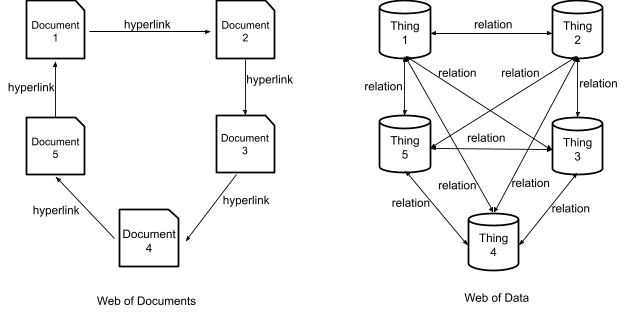
\includegraphics[width=\columnwidth]{images/ch2/semantic-web.png}
    \caption{Following Aghaei et al.~\cite{aghaei2012evolution},
    an illustration of the contrast between the web of documents
    that uses \ac{html} and the web of data that uses \ac{rdf}.
    \label{semantic-web}}
\end{figure}

\section{Linked Open Data}
\label{sec:linkedopendata}

Linked Open Data is the amalgamation of
linked data, that expresses the relationships between data,
and open data, that grants broad access rights to the data.
The relationships amongst data are equally important 
to the working of the semantic web 
as the access to the data itself~\cite{bizer2011linked}.

In 2006, 
Berners-Lee~\cite{bizer2009linked} 
described four basic rules 
for publishing and connecting 
structured datasets across the web. 
These rules have become known as the 
linked data 
principles, and have been enhanced by Berners-Lee, Bizer, Heath, 
and Idehen~\cite{bizer2009emerging, bizer2011linked, bizer2008linked, heath2011linked}.
Those rules are presented here. 
Terminology introduced in the rules is described in the subsequent text.

Rule 1.
Use \acp{uri} as unique names for (all) things on the web,
so that the same \ac{uri} used in different datasets is understood to signify
the same thing.

Rule 2.
Use \ac{https} (or \ac{http}) \acp{uri} to look up those unique names
because the hypertext transfer protocols allow easy retrieval of resources,
which promotes the publication and use of data on the web.

Rule 3.  
Provide useful information to others, using standards from the \ac{rdf} family,
in response to a look-up of a unique name associated with one of your \acp{uri}.
   
Rule 4.
Use other (existing) \acp{uri} in your data to encourage discovery of more relationships,
which promotes the global interconnection of data.

These principles encourage the
naming of subjects, predicates, and objects with 
\ac{https} \acp{uri}\footnote{\tt https://www.w3.org/TR/uri-clarification/} 
and providing useful information through the \ac{rdf} family of standards.
Berners-Lee introduced the concept of 5-star 
\ac{lod}\footnote{\tt https://www.w3.org/TR/ld-glossary/\#x5-star-linked-open-data}
to denote structured data on the web as \ac{rdf} wherein all identifiers are \ac{https} \acp{uri}
pointing to other useful data sources, with an open license for access.

\subsection{Uniform Resource Identifiers}
\label{subsec:uri}

Resources on the web, 
whether they are abstract (logical) or physical,
are identified by a unique string of ASCII characters known 
as a \ac{uri}.
As described by Berners-Lee et al.~\cite{RFC3986uri} 
in RFC 3986 (which became STD 66), 
this unique string is subject to guidelines and security considerations 
while defining the syntax for a generic \ac{uri} 
and a process for resolving \ac{uri} references. 
Berners-Lee et al.~\cite{RFC3986uri} 
characterized \ac{uri} by discussing the component terms.

Numerous advantages come from uniformity. 
Various types of resource identifier can be used
in the same context even when the means accessing those resources may vary. 
Semantic interpretation of standard syntactic rules is the same
across various types of resource identifiers. 
New types of resource identifiers can be introduced
without affecting how other identifiers are used. 
Existing resource identifiers can be reused in a variety of settings, 
enabling new applications or protocols to benefit from that 
widely-utilized set of resource identifiers.

A resource is anything that can be identified
by a \ac{uri}. The pages on a website are a recognizable example. 
A resource is not necessarily available via the web. 
It may correspond to a physical entity such as a person,
an abstract concept such as a relationship,
or a numeric quantity.

An identifier distinguishes an object from all other objects within its scope.
The purpose of an identifier is to distinguish one resource from all others.
An identifier is not required to define the identity of what is referenced, 
though this may be the true for some.
A system using \acp{uri} is neither required to access the resource identified
and for some there is no intention that they be accessed.
    
Berners-Lee et al.~\cite{RFC3986uri} defined the generic syntax of a \ac{uri} 
as shown in Figure~\ref{syntax-diagram}. 
A \ac{uri} comprises five components in sequence 
(see Examples~\ref{generic-uri} and~\ref{authority-uri}). 
It is not mandatory for a \ac{uri} to have all the components.
\begin{flalign}
    \text{\tt \ac{uri} = scheme: [//authority] path [?query] [\#fragment]} &&
    \label{generic-uri}
\end{flalign}
\noindent
The authority component comprises three elements, which are:
\begin{flalign}
    \text{\tt authority = [userinfo@] host [:port]} &&
    \label{authority-uri}
\end{flalign}

\begin{figure}[h]
    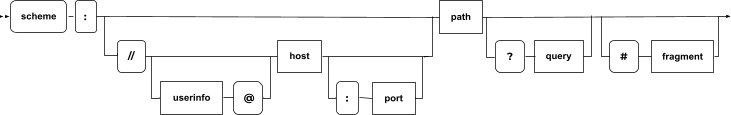
\includegraphics[width=\columnwidth]{images/ch2/syntax-diagram.png}
    \caption{Syntax diagram for a generic \ac{uri}, 
    after Berners-Lee et al.~\cite{RFC3986uri}.}
    \label{syntax-diagram}
\end{figure}
\noindent
One of the \acp{uri} from the Survey ontology is in Example~\ref{example-uri}.
Figure~\ref{components-of-uri-example} 
shows its components.
\begin{flalign}
    \text{\tt https://parita-amin.github.io/survey.owl\#Survey} &&
    \label{example-uri}
\end{flalign}

\begin{figure}[ht]
    \centering
    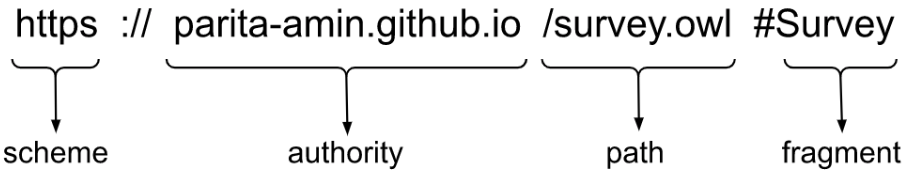
\includegraphics[width=\columnwidth]{images/ch2/components-of-uri-example.png}
    \caption{Components of the example \ac{uri}, 
    after Berners-Lee et al.~\cite{RFC3986uri}}
    \label{components-of-uri-example}
\end{figure}

\subsection{Resource Description Framework}
\label{subsec:rdf}

According to Flanders and Jannidis~\cite{julia2015data}, 
data modelling refers ``the process of representing data, 
their relationships, and their semantics in a way 
which is processable by humans and machines''. 
A data model is 
an abstract representation of data 
that standardizes how its components 
relate to one another and to the characteristics of real-world objects. 
Depending on the level of abstraction, 
there are three main types of data models, 
namely, 
conceptual, logical, and physical data model. 
Some widely-used primary data models are 
dimensional, relational, and \ac{er} models. 
RDF began as a metadata model and is now the means to describe resources 
(entities) and the relationships amongst them in a computer-understandable format, 
using basic data models like the \ac{er} model. 
An \ac{er} model is a high-level conceptual data model 
that assists rigorous analysis of the data requirements 
to build a well-designed database. 
The \ac{er} model depicts real-world entities and the relationships between them~\cite{lin2019structure}.

\ac{rdf} uses {\em properties} and {\em property values} 
to describe resources, which are named by \acp{uri}. 
The three types of objects in \ac{rdf} are resources, properties, and statements.
Each data object in a dataset on the web is considered a resource and is named 
using a \ac{uri}. 
The resources available on the web must be named using \ac{https} \acp{uri}. 
The \ac{w3c} has defined the 
{\tt rdf:type} 
property to represent the 
``object of one or more classes''~\cite{cyganiak2014rdf}. 
Resources are described by their characteristics, 
called {\em properties}. 
The object of \ac{rdf} 
that is used to combine a resource with a property of its value is a {\em statement}. 
A statement, 
in general terms, 
can be seen as building blocks of a statement in English, 
which are a subject, a predicate, and an object. 
An object in a statement can be either a property value, a resource, or a literal. 
\ac{rdf}, 
according to Beckett, Gandon and Schreiber~\cite{gandon2014rdf,zongmin2016rdf}, 
can be represented in three ways:
using \ac{xml} in an \ac{rdf}/\ac{xml} document,
as triples in subject-predicate-object form 
or in graphical form.

The University of Manchester has developed Pizza ontology 
which acts as an inspiration for ``pizza'' examples in this chapter.
Consider the following example:
\begin{flalign}  
    \text{\tt Pizza has CaloricContent with some integer value}&&
    \label{caloriccontent}
\end{flalign}
\noindent
Figure~\ref{rdf-xml-doc} shows the \ac{rdf}/\ac{xml},
which consists of various \ac{xml} tags.
An \ac{rdf}/\ac{xml} 
document starts and ends with {\tt <rdf:\ac{rdf}>} and 
{\tt </rdf:\ac{rdf}>} respectively.
    
\begin{figure}[h]
	\framebox{\vbox{\tt\small
        \begin{tabbing}
            \hspace*{0.5cm}\=\hspace*{0.5cm}\=\hspace*{0.5cm}\=\hspace*{0.5cm}\= \kill
            \hspace*{\columnwidth}\\[-1cm]
            @prefix rdf: <http://www.w3.org/1999/02/22-rdf-syntax-ns\#> .\\
            @prefix owl: <http://www.w3.org/2002/07/owl\#> .\\
            @prefix pizza: <http://www.semanticweb.org/pizzatutorial/ontologies/2020/ \\ \>\>\> PizzaTutorial\#> .\\
            @prefix xsd:  <http://www.w3.org/2001/XMLSchema\#> .\\
            <rdf:RDF>\\
            \><owl:Class rdf:about="pizza:Pizza">\\
            \>\>\><owl:onProperty rdf:resource="pizza:hasCaloricContent"/>\\
            \>\>\><owl:someValuesFrom rdf:resource="xsd:integer"/>\\
            \></owl:Class>\\
            </rdf:RDF>
            \\[-1cm]
        \end{tabbing}
      }}
      \caption{Example~\ref{caloriccontent} expressed as \ac{rdf}/\ac{xml}.}
      \label{rdf-xml-doc}
\end{figure}
     
{\tt http://www.semanticweb.org/pizzatutorial/ontologies/2020/PizzaTutorial\#},  
{\tt http://www.w3.org/1999/02/22-rdf-syntax-ns\#},  
{\tt http://www.w3.org/2002/07/owl\#}, and 
{\tt http://www.w3.org/2001/XMLSchema\#}
are the base \acp{uri} that have been expressed using prefixes 
{\tt pizza}, {\tt rdf}, {\tt owl}, and {\tt xsd} respectively 
for the classes and properties in Figure~\ref{rdf-xml-doc}. 
The resource being described is {\tt pizza:Pizza}, 
{\tt pizza:hasCaloricContent} is the property, and 
{\tt xsd:integer} is the value.

Figure~\ref{rdf-triple} 
shows an example of an \ac{rdf} triple, 
where {\tt pizza:Pizza} is the subject; 
the predicate is {\tt pizza:hasCaloricContent}; 
and the object is {\tt xsd:integer}. 

\begin{figure}[htp]
    \framebox{\vbox{\tt\small
    \begin{tabbing}
        \hspace*{0.9cm}\=\hspace*{0.9cm}\=\hspace*{0.9cm}\=\hspace*{0.5cm}\= \kill
        \hspace*{\columnwidth}\\[-1cm]
        Subject: {\tt pizza:Pizza}\\
        \>\>Predicate: {\tt pizza:hasCaloricContent}\\
        \>\>\>\>Object: {\tt xsd:integer}
        \\[-1cm]
    \end{tabbing}
    }}
    \caption{An illustration of Example~\ref{caloriccontent} as an \ac{rdf} triple.}
    \label{rdf-triple}
\end{figure}
  
Figure~\ref{rdf-graph} 
shows Example~\ref{caloriccontent} in graphical format. 
A resource is represented by an oval;
a property value is represented by a rectangle;
and a property is represented by an arrow,
to show that the property (predicate, {\tt pizza:hasCaloricContent}) 
connects the resource (subject, {\tt pizza:Pizza}) with the value (object, {\tt xsd:integer}).
    
\begin{figure}[htp]
    \centering
    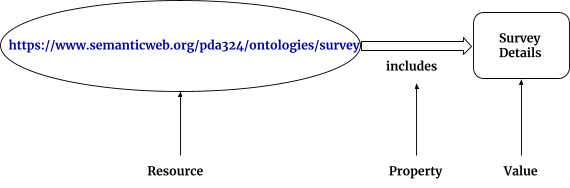
\includegraphics[width=\columnwidth]{images/ch2/rdf-graph.png}
    \caption{Graphical representation of Example~\ref{caloriccontent}.}
    \label{rdf-graph}
\end{figure}
    
The subject and object of an \ac{rdf} triple of \ac{rdf} act as nodes in the graph
where they are two entities and 
the predicate being the third entity acts as a connector between them. 
Considering an entity-relationship data model, 
the predicate can be treated as a relationship shared by the subject and the object. 
In addition to the \ac{rdf}/\ac{xml} and the line-based N-triples~\cite{beckett2014rdf} 
formats, 
the \ac{rdf} data model has a variety of serialization formats such as
\ac{turtle}; \ac{n3}, 
which is an extension of N-Triples (line based) 
and adds a graph label to each line 
that allows multiple graph encoding~\cite{cyganiak2008n}.

There can be more details added to Example~\ref{caloriccontent}
(illustrated in Figures~\ref{rdf-xml-doc},~\ref{rdf-triple}, and~\ref{rdf-graph}). 
That is, 
more statements can be added in relation to the original statement.  
Suppose the new statement added is: 
\begin{flalign}  
    \text{\tt Pizza has PizzaBase} &&
    \label{pizzabase}
\end{flalign}
\noindent
where the property (predicate, {\tt pizza:hasBase}) 
connects the resource (subject, {\tt pizza:Pizza}) with the value (object, {\tt pizza:PizzaBase}).
Figure~\ref{graph-for-relative-statements} shows a graphical representation
of the two example statements combined.

\begin{figure}[ht]
    \centering
    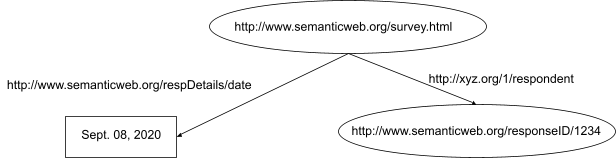
\includegraphics[width=\columnwidth]{images/ch2/graph-for-relative-statements.png}
    \caption{Graphical representation of Examples~\ref{caloriccontent} and~\ref{pizzabase} combined,
    following the \ac{rdf} Primer~\cite{manola2004rdf}.}
    \label{graph-for-relative-statements}
\end{figure}
\noindent
Adding more complexity to the system,
include a description of the types of {\tt PizzaBase}.
Figure~\ref{graph-for-base-types} 
shows a graphical representation of this system.
\begin{flalign}  
    \text{ {\tt DeepPanBase} and {\tt ThinAndCrispyBase}} &&
    \label{kindsofbase}
\end{flalign}

\begin{figure}[ht]
    \centering
    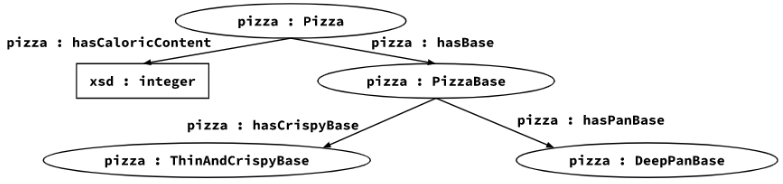
\includegraphics[width=\columnwidth]{images/ch2/graph-for-base-types.png}
    \caption{Graphical Representation of \ac{rdf} with types of PizzaBase, 
    after the \ac{rdf} Primer~\cite{manola2004rdf}.}
    \label{graph-for-base-types}
\end{figure}

{\tt pizza:Pizza} (subject) 
is connected to {\tt pizza:PizzaBase} (object) node 
through {\tt pizza:hasBase} (predicate). 
Further, 
the {\tt pizza:PizzaBase} node has multiple child nodes, 
namely, 
{\tt pizza:ThinAndCrispyBase} and {\tt pizza:DeepPanBase} 
where the \acp{uri} for the predicates are 
{\tt pizza:hasCrispyBase} and {\tt pizza:hasPanBase} respectively. 
Instead of using an unnecessary \ac{uri} 
for the {\tt pizza:PizzaBase} entity, 
a blank node can be used to denote the entity, 
as shown in Figure~\ref{blank-node-for-rdf}. 
As the relationships of the node with other nodes give sufficient details without hindering the flow of the data tree, 
the node does not require a 
\ac{uri} reference.

\begin{figure}[htp]
    \centering
    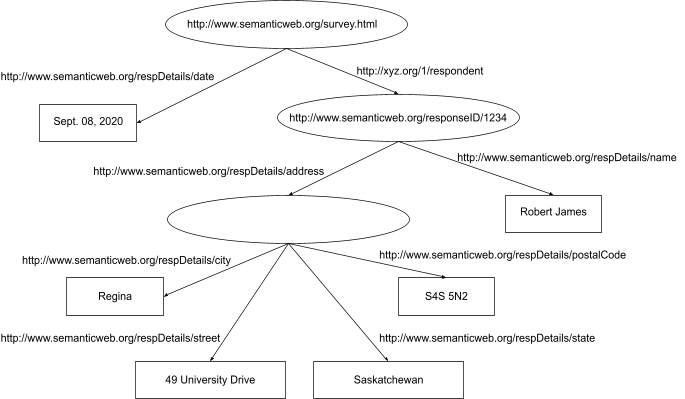
\includegraphics[width=\columnwidth]{images/ch2/blank-node-for-rdf.png}
    \caption{\ac{rdf} Representation in Figure~\ref{graph-for-base-types} 
    without a \ac{uri} (blank node) for PizzaBase Entity, after the \ac{rdf} 
    Primer~\cite{manola2004rdf}.}
    \label{blank-node-for-rdf}
\end{figure}

According to the \ac{w3c} 
Recommendation\footnote{\tt https://www.w3.org/TR/rdf11-concepts/},  
the design should 
``have a simple data model; 
formal semantics and provable inference; 
should use an extensible \ac{uri}-based vocabulary and an \ac{xml}-based syntax; 
should support the use of \ac{xml} schema datatypes; 
and should allow any one to make statements about any resource''. 

\ac{rdfs}, 
according to McBride~\cite{mcbride2004resource}, 
was introduced by the \ac{w3c} 
as a technique to define resource types and property names. 
The data publishers can use \ac{rdfs} 
to define various vocabularies in an \ac{rdf} model. 
Some of the commonly used \ac{rdfs} classes and properties\footnote{\tt https://www.w3.org/TR/rdf-schema/} 
along with their description are listed in Table~\ref{rdfs-classes-and-properties}~\cite{mcbride2004resource}.

\begin{table}[h!]
	\centering
    \begin{tabular}{| l | p{10cm} |} \hline
		Class/Property & Description  \\  \hline
     rdfs:Resource & All things described by \ac{rdf} are called resources  \\ \hline
     rdfs:Class & The class of resources that are \ac{rdf} classes \\ \hline
     rdf:Property & The class of \ac{rdf} properties. 
     It is an instance of rdfs:Class  \\ \hline
     rdfs:Literal & The class of literal values like integers and strings  \\ \hline
     rdfs:Datatype & The class of datatypes. All the objects of this class correspond to the \ac{rdf} model of datatype  \\ \hline
     rdf:HTML & The class of \ac{html} literal values and subclass of rdfs:Literal  \\ \hline
     rdfs:range & An instance of rdf:Property that is used to state that the values of a property are instances of one or more classes \\ \hline
     rdfs:domain & An instance of rdf:Property that is used to state that any resource that has a given property is an instance of one or more classes \\ \hline
     rdf:type & An instance of rdf:Property that is used to state that a resource is an instance of a class  \\ \hline
     rdfs:subClassOf & An instance of rdf:Property that is used to state that all the instances of one class are instances of another  \\ \hline
     rdfs:label & an instance of rdf:Property that may be used to provide a human-readable version of a resource's name  \\ \hline
     rdfs:subPropertyOf \ \ & An instance of rdf:Property that is used to state that all resources related by one property are also related by another  \\ \hline
    \end{tabular}
    \caption{Commonly used Classes and Properties of RDFS}
    \label{rdfs-classes-and-properties}
\end{table}

\subsection{Open Data}
\label{subsec:opendata}

According to the Open Knowledge Foundation~\cite{foundation}, 
``Open Data is data that can be freely used, 
re-used and redistributed by anyone - subject only, 
at most, 
to the requirement to attribute and share-alike''. 
To make open data available to everyone on the web, 
the data don't need to be interlinked. 
Important features of open data are:

\begin{itemize}

	\item Availability and access: 
	the data should be available on the web. 
  	The users should be able to access the data easily by downloading 
	them over the internet.
	It should be easy to access and modify the data.
  
  	\item Re-use and redistribution: 
	the data on the web must have permissions to re-use and 
	redistribute in combination to other datasets.
 
	\item Universal participation: 
	the data should be available to use, re-use, 
	and redistribute for all the users without any 
	discrimination to an individual or a group.
	
\end{itemize}

Linked data is concerned with publishing structured data,
along with the semantics of the relationships amongst that data,
onto the web.
The \ac{w3c} standards and technologies handle the distribution and 
engagement of this data across the web with the potential to present 
it as one huge database~\cite{bernerslee1999weaving}.

\subsection{Wikidata}
\label{subsec:wikidata}

A variety of projects and websites, 
that use linked open data, 
have been developed. 
Wikidata is one of the major projects of linked open data that present structured data on the semantic web. 

Krotzsch and Vrandecic~\cite{denny2014wikidata}
describe the introduction of Wikidata to the world in 2012. 
According to Erxleben et al.~\cite{fredo2014intro}, 
Wikidata is ``the community-created knowledge base of Wikipedia 
and the central data management platform for Wikipedia''. 
It was established for the collection and integration of Wikipedia data  
into
the semantic web. 
Wikidata is a free and open-source tool that handles a large amount of 
structured data and maintains pages that store the data. 
Each entity on Wikidata represents the subject of a triple with a dedicated page. 
The properties of Wikidata are similar to that of \ac{rdf} 
where the individuals and classes are indicated using items. 
Data on a page of the Wikidata is available for the users to access as well as edit.

For instance, 
the University of Regina (Q3104287) 
has an item page\footnote{\tt https://www.wikidata.org/wiki/Q3104287}.
Figure~\ref{wikidata-uofr} 
illustrates a portion of the contents of this page. 

\begin{figure}[htp]
    \centering
    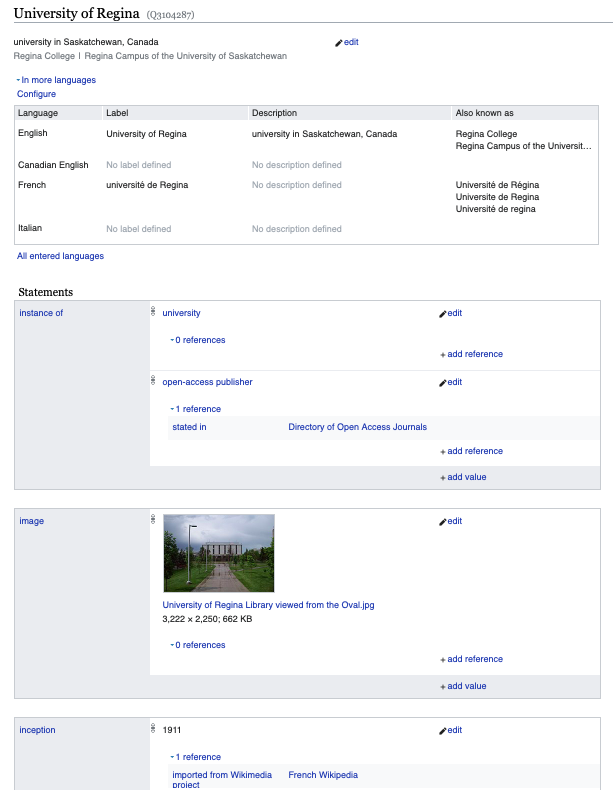
\includegraphics[width=\columnwidth]{images/ch2/wikidata-uofr.png}
    \caption{A portion of the item page for ``University of Regina'' on Wikidata.}
    \label{wikidata-uofr}
\end{figure}

Wikidata uses a method of automatically assigning unique identifiers to the entities, 
which are used as the labels of the item pages instead of the actual names of the entities. 
These identifiers are a string starting with a capital Q followed by a sequence of digits. 
The identifiers are assigned irrespective of the language as the Wikidata website supports multiple languages.

An item page on Wikidata consists of two main sections.
The first section, entitled Statements, contains a list properties and values.
The properties, along with their property IDs, used for the University of Regina 
are listed in Table~\ref{uofr-statement-properties-and-id}.
The other section is Identifiers, which consists of various IDs associated with the subject.
The identifiers, along with their property IDs, used for the University of Regina 
are listed in Table~\ref{uofr-identifier-properties-and-id} 
where as the \ac{rdf}/\ac{xml} 
description of the University of Regina on Wikidata is as shown in Figure~\ref{rdf-xml-uofr}. 
  
\begin{table}[h!]
        \centering
        \begin{tabular}{|l|l|} \hline 
             Statement Property \ & Property ID \\ \hline
             instance of & P31\\ \hline
             image & P18\\ \hline
             inception & P571\\ \hline
             country & P17\\ \hline
             located in the administrative territorial entity & P131\\ \hline
             coordinate location & P625\\ \hline
             subsidiary & P355\\ \hline
             official website & P856\\ \hline
             commons category & P373\\ \hline
             topic's main category & P910\\ \hline
             category for employees of the organization & P4195\\ \hline
             category for alumni of educational institution & P3876\\ \hline
             API endpoint & P6269\\ \hline
             social media followers & P8687\\ \hline
        \end{tabular}
        \caption{Statement Properties and Property IDs for ``University of Regina'' on Wikidata.}
        \label{uofr-statement-properties-and-id}
\end{table}
   
\begin{table}[h!]
	\centering
  	\begin{tabular}{|l|l|} \hline
	Identifier Property \ & Property ID \\ \hline
    VIAF ID & P214\\ \hline
    ISNI & P213\\ \hline
    GND ID & P227\\ \hline
    Library of Congress authority ID & P244\\ \hline
             WorldCat Identities & P7859\\ \hline
             ARWU university ID & P5242\\ \hline
             Crossref funder ID & P3153\\ \hline
             Facebook ID & P2013\\ \hline
             Freebase ID & P646\\ \hline
             Google Maps Customer ID & P3749\\ \hline
             GRID ID & P2427\\ \hline
             HAL structure ID & P6773\\ \hline
             LittleSis organization ID & P3393\\ \hline
             Microsoft Academic ID & P6366\\ \hline
             Ringgold ID & P3500\\ \hline
             ROR ID & P6782\\ \hline
             Times Higher Education World University ID & P5586\\ \hline
             Twitter username & P2002\\ \hline
             U-Multirank university ID & P5600\\ \hline
	\end{tabular}
    \caption{Identifier Properties and Property IDs for ``University of Regina'' on Wikidata.}
    \label{uofr-identifier-properties-and-id}
 \end{table}

\begin{figure}[htp]
    \framebox{\vbox{\tt\small
    \begin{tabbing}
        \hspace*{0.9cm}\=\hspace*{0.9cm}\=\hspace*{0.9cm}\=\hspace*{0.5cm}\= \kill
        \hspace*{\columnwidth}\\[-1cm]
        <?xml version="1.0" encoding="utf-8" ?>\\
        <rdf:RDF xmlns:rdf="http://www.w3.org/1999/02/22-rdf-syntax-ns\#"\\
        \>xmlns:xsd="http://www.w3.org/2001/XMLSchema\#"\\
        \>xmlns:ontolex="http://www.w3.org/ns/lemon/ontolex\#"\\
        \>xmlns:wdt="http://www.wikidata.org/prop/direct/"\\
        \>xmlns:wdtn="http://www.wikidata.org/prop/direct-normalized/">\\
        <rdf:Description rdf:about="https://www.wikidata.org/wiki/Special:EntityData/Q3104287">\\
        \><rdf:type rdf:resource="http://schema.org/Dataset"/>\\
        \><schema:about rdf:resource="https://www.wikidata.org/entity/Q3104287"/>\\
        \><cc:license rdf:resource="http://creativecommons.org/publicdomain/zero/1.0/"/>\\
        \><rdf:Description rdf:about="https://en.wikipedia.org/wiki/University\_of\_Regina">\\
        \>\><rdf:type rdf:resource="http://schema.org/Article"/>\\
        \>\><schema:about rdf:resource="http://www.wikidata.org/entity/Q3104287"/>\\
        \>\><schema:inLanguage>en</scehma:inLanguage>\\
        \>\><schema:isPartOf rdf:resource="https://en.wikipedia.org/"/>\\
        \>\><schema:name xml:lang="en">Univeristy of Regina</schema:name>\\
        \>\><schema:description xml:lang="en">university in Saskatchewan, Canada\\\>\></schema:description>\\
        \>\><wdt:P18 rdf:resource="http://commons.wikinedia.org/wiki/Special:FilePath/\\ \>\>University\%20of\%20Regina\%20Library\%20viewed\%20from\%20the\%20Oval.jpg"/>\\
        \></rdf:Description>\\
        </rdf:Description>\\
        </rdf:RDF>
        \\[-1cm]
    \end{tabbing}
    }}
    \caption{Wikidata Entry (RDF/XML) for ``University of Regina''.}
    \label{rdf-xml-uofr}
\end{figure}

\section{Ontology in Web Semantics}
\label{sec:ontologyinwebsemantics}

Ontology is a branch of information science 
that encloses representation, nomenclature, and 
definition of various properties, categories, and relationships shared among 
entities, which includes all types of data, concepts and entities,
that support any number of domains 
in which the user is interested.
In other words, 
ontology is a form of defining a set of concepts for representing the subject 
properties and the relationships shared among them. 
According to Gruber~\cite{gruber1995towards}, 
ontology is 
{\tt an explicit specification of a conceptualization}, 
where conceptualization is 
``an abstract, simplified view of the world 
(includes objects, concepts and other entities 
that are assumed to exist in some area of interest and the relationships 
that hold among them) 
that we wish to represent for some purpose''. 
In web semantics, 
an ontology is used to define the semantics of the resources briefly and methodically. 
On the semantic web, 
the ontologies have been used 
to define resources' conceptual and physical qualities 
in the form of metadata schema for a predetermined group of users.

\subsection{OWL Ontologies}
\label{subsec:owlontologies}

The \ac{w3c} developed a standard ontology language called 
\ac{owl}\footnote{\tt https://www.w3.org/TR/owl-overview/} 
to define and describe concepts for ontology
using different facilities and operations like intersection, union and negation. 
It is based on a logical model 
on which a reasoner 
can be used to check the mutual consistency 
among the statements and definitions in the ontology. 
The reasoner is also responsible for the identification of a 
suitable concept for particular definitions~\cite{horridge2009practical}.

\subsection{Components of OWL Ontologies}
\label{subsec:componentsofowlontologies}

An \ac{owl} ontology consists of a set of components that define and describe the concepts collectively. 
The basic components of any \ac{owl} ontology, 
Individuals, Properties and Classes, 
are briefly explained in this section.

\subsubsection{Individuals}
\label{subsubsec:individuals}

According to Horridge et al.~\cite{horridge2009practical}, 
``Individuals represent objects in the domain in which we are interested''. 
Individuals are the objects of classes. 
Figure~\ref{owl-individuals} 
shows the representation of different individuals in various domains. 
The triangles are used here to denote the individuals in free space.

\begin{figure}[htp]
    \centering
    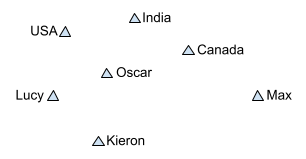
\includegraphics[width=8cm]{images/ch2/owl-individuals.png}
    \caption{Representation of Individuals in OWL}
    \label{owl-individuals}
\end{figure}

\subsubsection{Properties}
\label{subsubsec:properties}

Binary relationships, links shared by two individuals (things),
are called properties. 
For instance, 
the individuals 
{\tt Customer1} and {\tt AmericanaPizza1} from Figure~\ref{owl-individuals} 
are linked to each other by the property {\tt purchasedPizza}. 
Each property can have its inverse. 
For instance, 
{\tt purchasedPizza} 
can have an inverse property {\tt purchasedBy}. 
The properties can be symmetric or transitive. 
It is possible to have functional properties where the properties can be restricted to having only one value.

Figure~\ref{owl-properties} 
shows representation of properties between the individuals {\tt Customer1} and {\tt Medium}, 
and {\tt Customer1} and {\tt AmericanaPizza1}. 
The relation between {\tt Customer1} and {\tt Medium} is {\tt hasSpicinessPreference}. 
The arrow between two individuals in the figure denotes the property (relationship) between them.

\begin{figure}[htp]
    \centering
    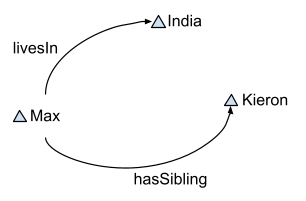
\includegraphics[width=8cm]{images/ch2/owl-properties.png}
    \caption{Representation of Properties in OWL}
    \label{owl-properties}
\end{figure}

\subsubsection{Classes}
\label{subsubsec:classes}

In \ac{owl}, 
the sets consisting of individuals are called \ac{owl} classes. 
Mathematical (formal) descriptions are used to describe the \ac{owl} classes. 
These descriptions include accurate statements on the requirements for the class membership. 
For instance, 
the class {\tt Customer} 
consists of all the individuals that are customers in the Domain of Discourse 
which can contain one or more classes. 
Inheritance in \ac{owl} classes (Class Hierarchy) 
may exist with the classes having subclasses and/or super-classes which is technically termed as taxonomy. 
``Subclasses specialise (``are subsumed by'') their super-classes''~\cite{horridge2009practical}. 
For instance, 
consider the classes {\tt Person} and {\tt Customer} from the pizza ontology, 
where {\tt Customer} is a subclass of {\tt Person}.
This implies the following statements:

\begin{itemize}

    \item All customers are person
    
    \item All members of class {\tt Customer} are members of class {\tt Person}
    
    \item Being a {\tt Customer} implies that individual is {\tt Person}
    
    \item {\tt Customer} is subsumed by {\tt Person}
    
\end{itemize}

Figure~\ref{owl-classes-with-individuals-and-properties} 
shows the representation of the classes 
for the individuals and properties that are 
shown in Figure~\ref{owl-properties}.

\begin{figure}[htp]
    \centering
    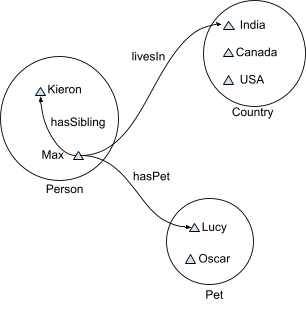
\includegraphics[width=8cm]{images/ch2/owl-classes-with-individuals-and-properties.png}
    \caption{Representation of OWL Classes Consisting of Individuals and Properties}
    \label{owl-classes-with-individuals-and-properties}
\end{figure}

\subsection{Ontology Editors}
\label{subsec:ontologyeditors}

Ontology editors are used by publishers 
to create new ontologies 
when the existing vocabulary is not suitable for their purpose. 
A list of ontology editors\footnote{\tt https://www.w3.org/wiki/Ontology\_editors} 
that can be used to edit, manage, organize and visualize ontology 
includes Protégé, NeOn Toolkit, SWOOP, Neologism, TopBraid Composer, 
Vitro, Knoodl, Anzo for Excel, OWLGrEd, Fluent Editor, Semantic Turkey, VocBench. 
Protégé is the most popular ontology editor among researchers. 
Most of the editors from the list are 
either non-existent or 
there exists negligible information about them, 
which has driven the decision of the use of protégé 
for ontology development which is discussed in detail in Chapter~\ref{chap:proofOfConcept}.

\section{Linked Data Life Cycle}
\label{sec:linkeddatalifecycle}

The Linked Data Life Cycle includes multiple stages as described by 
Ngomo et al.~\cite{ngomo2014introduction} 
which are listed in
Table~\ref{ldlc-stages}.
Each stage of this life cycle is independent yet linked to one another. 
So, 
it is not mandatory to go through all the stages sequentially 
to publish the data on the web. 
It is necessary to use a procedure that follows the life cycle 
to ensure the quality of data to be published as linked data. 
The first stage, 
generally, 
is data extraction along with conversion of the extracted data 
(in forms other than \ac{rdf}) into \ac{rdf}. 
Once the data is in \ac{rdf} form, 
any or all of the other stages listed in 
Table~\ref{ldlc-stages} 
can be performed.

\begin{table}[h!]
    \centering
    \begin{tabular}{|l|p{10cm}|} \hline 
     Stage & Description \\ \hline
     Extraction & Extraction and conversion of unstructured and semi-structured data into \ac{rdf}\\ \hline
     Storage \& Querying & Storing the \ac{rdf} data in a format that supports data querying efficiently\\ \hline
     Authoring & Allowing the users to create new data or to access and 
     modify the existing data\\ \hline
     Linking & Creating links among the data belonging to various domains and users based on their entities\\ \hline
     Enrichment & Data enrichment for efficient query support using various top-tier structures\\ \hline
     Quality Analysis & Managing data using different strategies to ensure good quality of available data on the web\\ \hline
     Browsing \& Exploration & Making the structured data available on the web for the users to browse and explore effectively\\ \hline
    \end{tabular}
    \caption{Stages in Linked Data Life Cycle, after Ngomo et al.~\cite{ngomo2014introduction}}
    \label{ldlc-stages}
\end{table}

The linked data life cycle is too basic and generic 
and may not be the best approach for describing data semantics. 
While working on this research, 
it was established that the life cycle~\cite{ngomo2014introduction} 
has gaps and does not aid the development of 5-star \ac{lov}.
Hence, this thesis introduces a new approach in Chapter~\ref{chap:methodology} 
that can be followed for developing \ac{lov} to map CSV data.

\section{Conversion of Data from Spreadsheets to RDF}
\label{sec:csvtordf}

The preferred format of the data published on the semantic web is \ac{rdf} format. 
Many data scientists use tables and spreadsheets to store and publish data using CSV
files over \ac{rdf} format 
as conversion of data to \ac{rdf} 
is comparatively difficult. 
The data used by Dr. Hepting has been stored in tabular format which can be converted into \ac{rdf} 
using different open source tools~\cite{ermilov2013csv} 
listed by \ac{w3c}\footnote{\tt https://www.w3.org/wiki/ConverterToRdf} 
or using \ac{rml}\footnote{\tt https://d2s.semanticscience.org/docs/convert-rml/}. 

\subsection{Tools to Describe CSV Data using Vocabulary}
\label{subsec:tools}

%Some of the open-source tools listed by the \ac{w3c} 
%for the mapping of CSV data using \ac{lov} are
%OpenRefine, RDF123, csv2rdf4lod, XLWrap, and Tarql.
%After an extensive research on these tools, 
%OpenRefine has been used in this thesis as most of these tools are out-dated.

%\subsubsection{OpenRefine}
%\label{subsubsec:openrefine}
%
%OpenRefine\footnote{\tt https://openrefine.org}, 
%an \ac{rdf} extension of Google Refine, 
%is a Java-based set of tools that work with messy data using \ac{grel}
%It allows the users to extract, transform, export, and convert 
%CSV, Excel, spreadsheets and other tabular data into \ac{rdf} 
%where a GUI (Graphical User Interface) is used to define schema mapping. 

\begin{itemize}
   
    \item OpenRefine:
    
    OpenRefine\footnote{\tt https://openrefine.org}, 
    an \ac{rdf} extension of Google Refine, 
    is a Java-based set of tools that work with messy data using \ac{grel}
    It allows the users to extract, transform, export, and convert 
    CSV, Excel, spreadsheets and other tabular data into \ac{rdf} 
    where a GUI (Graphical User Interface) is used to define schema mapping. 
   
    \item RDF123:
    
    RDF123\footnote{\tt https://ebiquity.umbc.edu/resource/html/id/237/RDF123-java-application-v1-0} 
    is a Java application and servlet for the conversion of CSV 
    and spreadsheets to \ac{rdf} 
    which uses arbitrary graphs to define schema mapping. 
    According to Han et al.~\cite{han2008rdf}, 
    it uses a graphical RDF123 template to allow users to convert the data from spreadsheets to \ac{rdf}.
   
    \item csv2rdf4lod:
   
    csv2rdf4lod\footnote{\tt https://github.com/timrdf/csv2rdf4lod-automation/wiki} 
    is a tool that is used for the conversion of tabular data into structured and linked \ac{rdf} 
    using specifications that are based on declarative \ac{rdf} 
    enhancement parameters. 
    It forms default namespaces for \acp{uri} 
    and provides VoID and original metada for the conversion 
    using identifiers for source organization, dataset and version.
   
    \item XLWrap:
    
    XLWrap\footnote{\tt https://xlwrap.sourceforge.io} 
    is a graphical template based application that allows execution of various \ac{sparql} 
    queries~\cite{andreas2009xlwrap}. 
    The spreadsheets are wrapped to arbitrary \ac{rdf} 
    graphs which allows:
   
        \begin{itemize}
    	
	        \item Streamed processing of tabular data like Excel, OpenDocument and CSV
	
	        \item Loading Local/\ac{http}
	
	        \item Expressions that include calculator operations for Excel and OpenDocument, and Custom functions
	
	        \item Use of \ac{api} and \ac{sparql} endpoint
    
        \end{itemize}
   
    \item Tarql:
   
    Tarql\footnote{\tt https://tarql.github.io} 
    operates as a command-line application for the conversion of CSV to \ac{rdf} 
    using a user-defined mapping that is written in \ac{sparql} standard 1.1.
    
\end{itemize}

After an extensive research on these tools, 
OpenRefine has been used in this thesis as most of these tools are out-dated.
Also, the community of data scientists is more interested in developing more stable methods like using RMLConversion to map CSV data.

\subsection{Conversion Using RML}
\label{subsec:rmlconversion}

``An \ac{rml} mapping defines a mapping from any logical source to \ac{rdf}. 
It is a structure that consists of one or more triples maps.''\footnote{\tt https://rml.io/specs/rml/\#example-XML} 
The \ac{rml} rules can be written and tested using tools like the Matey Web UI\footnote{\tt https://rml.io/yarrrml/matey/}.

\subsubsection{Tools for RML Conversion}
\label{subsubsec:rmlconversiontools}

Once the \ac{rml} rules have been defined, 
the next step is generate \ac{rdf} 
from the \ac{rml} mappings. 
The list below shows multiple tools, 
suggested by Data2Services\footnote{\tt https://d2s.semanticscience.org/}, 
with various efficiency, stability, and features 
that can be used for \ac{rml} conversion.

\begin{itemize}
   
    \item RMLMapper:
    
    RMLMapper\footnote{\tt https://github.com/RMLio/rmlmapper-java} 
    is a reference implementation written in Java. 
    It supports custom functions and operations 
    with small files as it loads all data in memory. 
    
    \item RMLStreamer: 
    
    RMLStreamer\footnote{\tt https://github.com/RMLio/RMLStreamer}, 
    written in Scala, 
    is well-suited for large input files and 
    continuous data streams like sensor data. 
    It is still under development resulting in limited support 
    for the use of custom functions.    
    
    \item SDM-RDFizer:
    
    SDM-RDFizer\footnote{\tt https://github.com/SDM-TIB/SDM-RDFizer}, 
    written in Python, 
    implements optimized data structures and relational algebra operators 
    that enable an efficient execution of \ac{rml} 
    triple maps even in the presence of Big data. 
    A separate tools called Dragoman\footnote{\tt https://github.com/SDM-TIB/Dragoman} 
    can be used for the execution of custom functions.
    
    \item Morph-KGC:
    
    Morph-KGC\footnote{\tt https://morph-kgc.readthedocs.io/en/latest/documentation/} 
    is an \ac{rml} 
    conversion tool written in Python. 
    It does not support custom functions.
    
    \item RocketRML:
    
    RocketRML\footnote{\tt https://github.com/semantifyit/RocketRML} 
    is a JavaScript implementation for \ac{rml} conversion. 
    It provides an easy way to define custom functions.
        
\end{itemize}

\end{doublespace}
%!TEX root = parita-msc.tex
\chapter{Methodology}\label{chap:methodology}

\begin{doublespace}

This chapter focuses on the methodology involved in describing and publishing linked open data. Chapter~\ref{chap:proofOfConcept} presents proof of concept of this methodology.

\section{Workflow}

owl ontology -> csv to rdf -> license and publish

\end{doublespace}
%!TEX root = parita-msc.tex

\chapter{Proof of Concept}\label{chap:proofOfConcept}

\begin{doublespace}

Chapter~\ref{chap:methodology} focuses on the methodology which has been followed to describe and publish the linked open vocabulary for survey in this chapter.

\section{OWL Ontology for Survey Using Protégé}

Figure~\ref{feedback-form} shows the student feedback form for which the new vocabularies are described. 

\begin{figure}[htp]
    \centering
    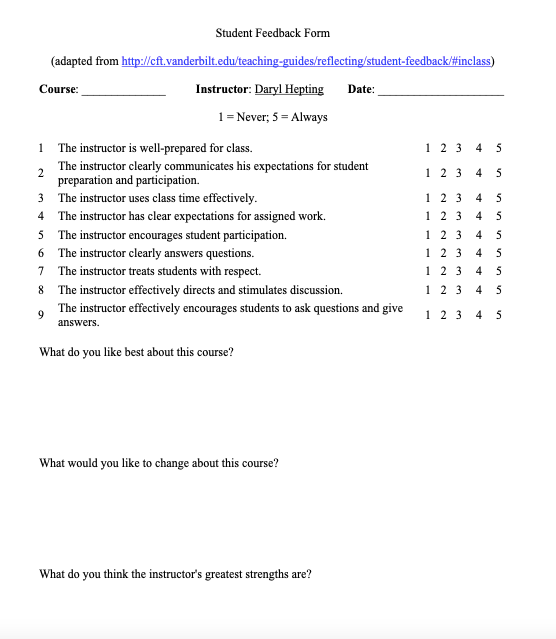
\includegraphics[width=15cm]{images/ch4/survey/feedback-form.png}
    \caption{The Student Feedback Form, from Hepting~\cite{prof}}
    \label{feedback-form}
\end{figure}

\subsection{Classes for Survey Ontology}

All the classes can be created and described using the steps described in section~\ref{subsec:classhierarchy}. The resultant class hierarchy for the survey ontology would be as shown in Figure~\ref{survey-class-hierarchy}. A survey can have \say{Survey Response}, \say{Respondent}, \say{Response Date}, \say{Type of Survey}, \say{Survey Questions}, and \say{Survey Answers}, which are considered for this ontology as well. 

\begin{figure}[htp]
    \centering
    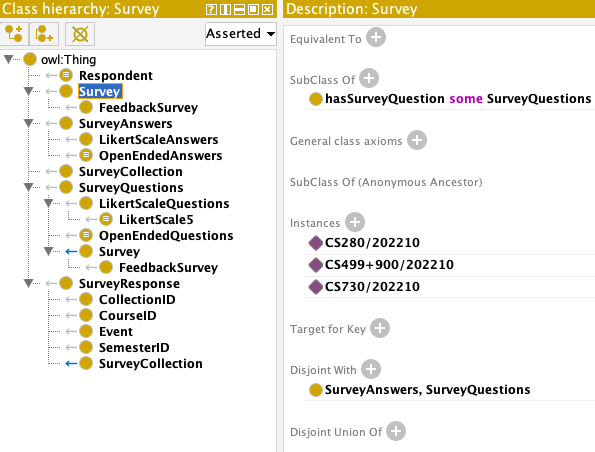
\includegraphics[width=15cm]{images/ch4/survey/survey-class-hierarchy.png}
    \caption{Class Hierarchy in Survey Ontology}
    \label{survey-class-hierarchy}
\end{figure}

Here, the type of survey used is feedback survey (\say{FeedbackSurvey} class). The \say{SurveyCollection} class corresponds to a collection of survey responses (\say{SurveyResponse} class) that were collected for a particular course (\say{CourseID} class) in a particular semester (\say{SemesterID} class) with a specific collection ID (\say{CollectionID} class). Furthermore, the survey questions and survey answers have classes corresponding to various forms of question-answer. Generally, feedback surveys consist of two types of questions, namely, \say{Likert Questions} and \say{Open-ended Questions}. The type of questions might differ depending on the designer of the survey, some of which, as stated on the \emph{SurveyMonkey}\footnote{https://www.surveymonkey.com/mp/survey-question-types/} website, are listed below. 

\begin{multicols}{2}
\begin{itemize}
   
    \item Multiple Choice Questions
   
    \item Rating Scale Questions
   
    \item Likert Scale Questions
   
    \item Matrix Questions
   
    \item Dropdown Questions
   
    \item Open-ended Questions
   
    \item Demographic Questions
   
    \item Ranking Questions
   
    \item Image Choice Questions
   
    \item Click Map Questions
   
    \item File Upload Questions
   
    \item Slider Questions
   
    \item Benchmarkable Questions

\end{itemize}
\end{multicols}

The feedback survey in this research has Likert and Open-ended questions. The classes described for the questions and answers are \say{LikertScaleQuestions}, and \say{OpenEndedQuestions} as sub-classes of \say{SurveyQuestions}, and \say{LikertScaleAnswers}, and \say{OpenEndedAnswers} as sub-classes of \say{SurveyAnswers}. For all the survey questions, there is a question and an answer, where both of them are considered as distinct classes. Open-ended questions have unpredictable answers.

\subsubsection{The ``LikertScaleQuestions'' Class}

Likert questions are the questions for which the answers are from the preset list of answers. For the Likert questions, the questions can be either of type \say{Never-Always-4} or \say{Never-Always-5} or \say{Never-Always-7} or \say{Never-Always-*}, of which Never-Always-5 has been used by Hepting~\cite{prof}. The survey ontology consists of \say{LikertScaleQuestions} class for likert questions.

In a Never-Always-5 type of survey, 5 degrees of agreement can be used. It is challenging to decide whether the range for the degrees would be 0 to 4, 1 to 5, 10 to 50, or something else. The degree of agreements used here are as shown in Table~\ref{likert-degrees}. In addition to these degrees, this ontology also considers the instances where the question wouldn't be answered. In this case, the field corresponding to the answer is left blank.

\begin{table}[h!]
    \centering
    \begin{tabular}{|c|l|}
    \hline Number \ & Agreement \\ \hline
     1 & Never\\ \hline
     2 & [Rarely]\\ \hline
     3 & [Sometimes]\\ \hline
     4 & [Often]\\ \hline
     5 & Always\\ \hline
    \end{tabular}
    \caption{Degrees of Agreement for Likert-scale Questions}
    \label{likert-degrees}
\end{table}

The \say{LikertScaleQuestions} class of survey ontology has a sub-class, \say{LikertScale5}, which represents the likert scale with the degrees of agreement from Table~\ref{likert-degrees}. The \say{Equivalent To} (from the description view of the class tab) can be used to describe the \say{LikertScale5} class in terms of a range containing degrees of agreement as shown in Figure~\ref{likertscale5-class}. Each of these degrees are treated as an individual (section~\ref{subsec:individuals}) of the class.

\begin{figure}[htp]
    \centering
    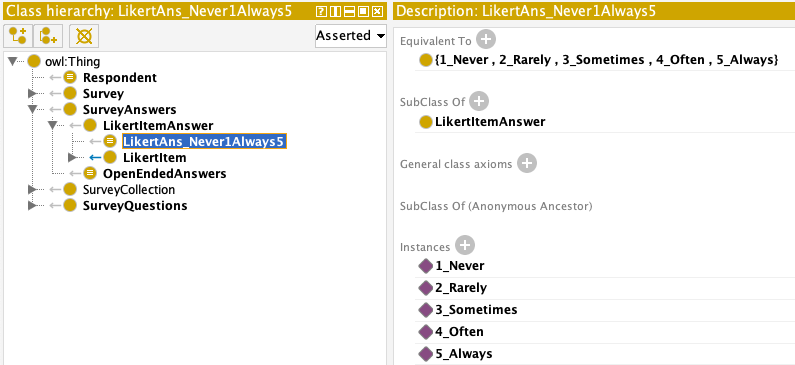
\includegraphics[width=15cm]{images/ch4/survey/likertscale5-class.png}
    \caption{``LikertScale5'' class in Survey Ontology}
    \label{likertscale5-class}
\end{figure}

\subsection{Object Properties for Survey Ontology}

Using the method of naming and building object properties described in section~\ref{subsec:objectproperties}, some of the primary object properties are described for the survey ontology as shown in Figure~\ref{survey-object-properties} where as Table~\ref{survey-object-properties-domains-and-ranges} shows the list of the object properties along with their domain and range classes. Table~\ref{survey-object-properties-parent-nodes-and-inverse} consists of the parent nodes and inverse properties of the object properties. The three parent nodes involved in object property hierarchy are \say{owl:TopObjectProperty}, \say{hasContent}, and \say{isContentOf}.

\begin{figure}[htp]
    \centering
    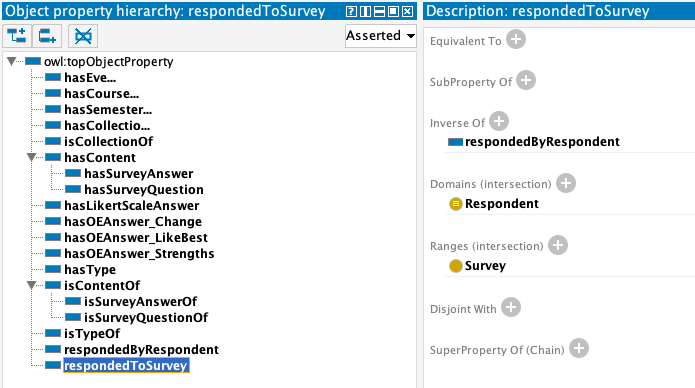
\includegraphics[width=15cm]{images/ch4/survey/survey-object-properties.png}
    \caption{Object Property Hierarchies, Domain and Range for Classes}
    \label{survey-object-properties}
\end{figure}

\begin{table}[h!]
    \centering
    \begin{tabular}{|l|l|l|} 
    \hline \ \ \ \ \ Object Property & \ \ \ \ \ \ \ \ Domain & \ \ \ \ \ \ \ \ Range\\ \hline
     hasSurveyQuestion & Survey & SurveyQuestions\\ \hline
     hasSurveyAnswer & Survey & SurveyAnswers\\ \hline
     hasOEAnswer\_Change & OpenEndedQuestions & OpenEndedAnswers\\ \hline
     hasOEAnswer\_LikeBest & OpenEndedQuestions & OpenEndedAnswers\\ \hline
     hasOEAnswer\_Strengths & OpenEndedQuestions & OpenEndedAnswers\\ \hline
     hasLikertScaleAnswer & LikertScaleQuestions & LikertScale5\\ \hline
     hasEvent & SurveyResponse & Event\\ \hline
     hasCourseID & SurveyResponse & CourseID\\ \hline
     hasSemesterID & SurveyResponse & SemesterID\\ \hline
     hasCollectionID & SurveyResponse & CollectionID\\ \hline
     isCollectionOf & SurveyCollection & SurveyResponse\\ \hline
     respondedToSurvey & Respondent & Survey\\ \hline
     isTypeOf & FeedbackSurvey & Survey\\ \hline
    \end{tabular}
    \caption{Object Properties and Their Domain and Range}
    \label{survey-object-properties-domains-and-ranges}
\end{table}

\begin{table}[h!]
    \centering
    \begin{tabular}{|l|l|l|} 
    \hline \ \ \ \ \ Object Property & \ \ \ \ \ \ \ Parent Node & \ \ \ \ \ Inverse Property\\ \hline
     hasContent & owl:TopObjectProperty & isContentOf\\ \hline
     isContentOf & owl:TopObjectProperty & hasContent\\ \hline
     hasType & owl:TopObjectProperty & isTypeOf\\ \hline
     isTypeOf & owl:TopObjectProperty & hasType\\ \hline
     hasLikertScaleAnswer & owl:TopObjectProperty & \\ \hline
     hasOEAnswer\_Change & owl:TopObjectProperty & \\ \hline
     hasOEAnswer\_LikeBest & owl:TopObjectProperty & \\ \hline
     hasOEAnswer\_Strengths & owl:TopObjectProperty & \\ \hline
     hasEvent & owl:TopObjectProperty & \\ \hline
     hasCourseID & owl:TopObjectProperty & \\ \hline
     hasSemesterID & owl:TopObjectProperty & \\ \hline
     hasCollectionID & owl:TopObjectProperty & \\ \hline
     isCollectionOf & owl:TopObjectProperty & \\ \hline
     respondedByRespondent & owl:TopObjectProperty & respondedToSurvey\\ \hline
     respondedToSurvey & owl:TopObjectProperty & respondedByRespondent\\ \hline
     hasSurveyQuestion & hasContent & isSurveyQuestionOf\\ \hline
     hasSurveyAnswer & hasContent & isSurveyAnswerOf\\ \hline
     isSurveyQuestionOf & isContentOf & hasSurveyQuestion\\ \hline
     isSurveyAnswerOf & isContentOf & hasSurveyAnswer\\ \hline
    \end{tabular}
    \caption{Object Properties with Their Parent Nodes and Inverse Properties}
    \label{survey-object-properties-parent-nodes-and-inverse}
\end{table}

\subsection{Data Properties for Survey Ontology}

Data properties for survey ontology have been described following the method described in section~\ref{subsec:dataproperties} which are as shown in Figure~\ref{survey-data-properties}.

\begin{figure}[htp]
    \centering
    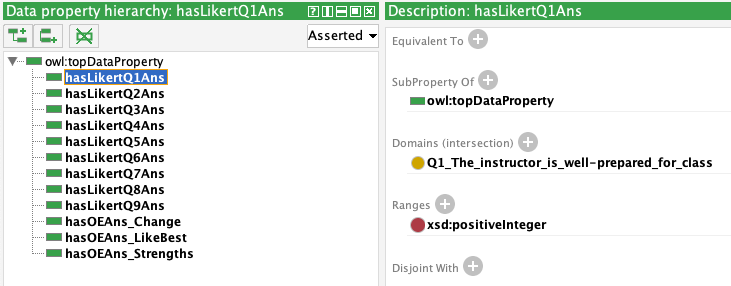
\includegraphics[width=15cm]{images/ch4/survey/survey-data-properties.png}
    \caption{Data Property Hierarchies, Domain and Range for Classes}
    \label{survey-data-properties}
\end{figure}

The parent node of all the data properties is \say{owl:topDataProperty} and the domain and range for all the data properties are listed in Table~\ref{survey-data-properties-domains-and-ranges}. The properties for likert answers restrict the datatype to positive integer and to string for open-ended answers.

\begin{table}[h!]
    \centering
    \begin{tabular}{|l|l|l|} 
    \hline \ \ \ \ \ \ \ \ \ \ \ \ \ \ \ Data Property &\ \ \ Domain &\ \ \ \ \ \ \ Range\\ \hline
     hasLikertAns\_is\_well-prepared\_for\_class & Respondent & xsd:positiveInteger\\ \hline
     hasLikertAns\_clearly\_communicates\_his\_expecta-&\\ tions\_for\_student\_preparation\_and\_participation & \multirow{-2}{5em}{Respondent} & \multirow{-2}{8.5em}{xsd:positiveInteger}\\ \hline
     hasLikertAns\_uses\_class\_time\_effectively & Respondent & xsd:positiveInteger\\ \hline
     hasLikertAns\_has\_clear\_expectations\_for&\\ \_assigned\_work & \multirow{-2}{5em}{Respondent} & \multirow{-2}{8.5em}{xsd:positiveInteger}\\ \hline
     hasLikertAns\_encourages\_student\_participation & Respondent & xsd:positiveInteger\\ \hline
     hasLikertAns\_clearly\_answers\_questions & Respondent & xsd:positiveInteger\\ \hline
     hasLikertAns\_treats\_students\_with\_respect & Respondent & xsd:positiveInteger\\ \hline
     hasLikertAns\_effectively\_directs\_and\_stimulates&\\ \_discussion & \multirow{-2}{5em}{Respondent} & \multirow{-2}{8.5em}{xsd:positiveInteger}\\ \hline
     hasLikertAns\_effectively\_encourages\_students\_to&\\ \_ask\_questions\_and\_give\_answers & \multirow{-2}{5em}{Respondent} & \multirow{-2}{8.5em}{xsd:positiveInteger}\\ \hline
     hasOEAnswer\_Change & Respondent & xsd:string\\ \hline
     hasOEAnswer\_LikeBest & Respondent & xsd:string\\ \hline
     hasOEAnswer\_Strengths & Respondent & xsd:string\\ \hline
    \end{tabular}
    \caption{Data Properties and Their Domain and Range}
    \label{survey-data-properties-domains-and-ranges}
\end{table}

\subsection{Individuals}\label{subsec:individuals}

While dealing with ontologies, an instance of class is termed as an \say{Individual}. In protégé, an individual can be described as an instance of class using the Description view of the Class tab. For example, Figure~\ref{instances-of-survey-class} shows instances of \say{Survey} class.

\begin{figure}[htp]
    \centering
    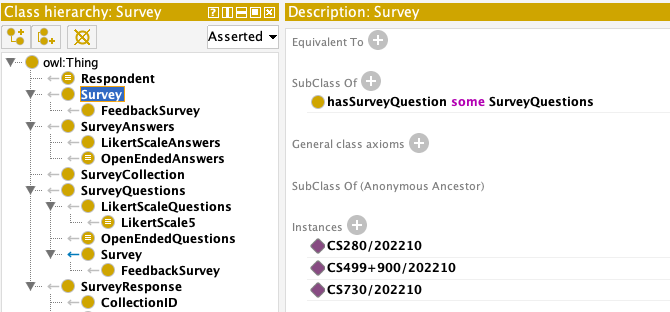
\includegraphics[width=15cm]{images/ch4/survey/instances-of-survey-class.png}
    \caption{Individuals for Survey Class}
    \label{instances-of-survey-class}
\end{figure}

A new individual can be described using the Individuals view of the Entities tab where as the property assertions view can be used to describe the property restrictions. Table~\ref{survey-individuals} shows a list of classes and individuals described in survey ontology.

\begin{table}[h!]
    \centering
    \begin{tabular}{|l|l|} 
    \hline \ \ \ \ \ \ \ \ \ \ Class & \ \ \ \ \ \ \ \ \ \ \ \ \ \ \ \ \ \ \ \ \ \ \ \ \ \ \ \ \ Individuals \\ \hline
     Respondent &  1, 2, 3, ... , 59 \\ \hline
     Survey & CS280/202210, CS499+900/202210, CS730/202210 \\ \hline
     SurveyCollection &  Collection1, Collection2 \\ \hline
     Event &  FinalExam, Midterm \\ \hline
     CollectionID &  CS280/202210/Collection1 \\ \hline
     SemesterID &  202210, 202220, 202230 \\ \hline
     CourseID &  CS280, CS499+900, CS730 \\ \hline
     \multirow{2}{9.5em}{OpenEndedQuestions} &  OEQuestion\_LikeBest, OEQuestion\_Change, \\& OEQuestion\_Strengths \\ \hline
     OpenEndedAnswers & OEAns\_LikeBest, OEAns\_Change, OEAns\_Strengths \\ \hline
     LikertScale5 & 1\_Never, 2\_Rarely, 3\_Sometimes, 4\_Often, 5\_Always \\ \hline
    \end{tabular}
    \caption{Classes and their Individuals}
    \label{survey-individuals}
\end{table}

\subsection{Final Class Hierarchy for Survey Ontology}

The final class hierarchy of the \ac{owl} ontology in protégé, after using the HermiT 1.4.3.456 reasoner, would be as shown in Figure~\ref{final-survey-classes}.

\begin{figure}[htp]
    \centering
    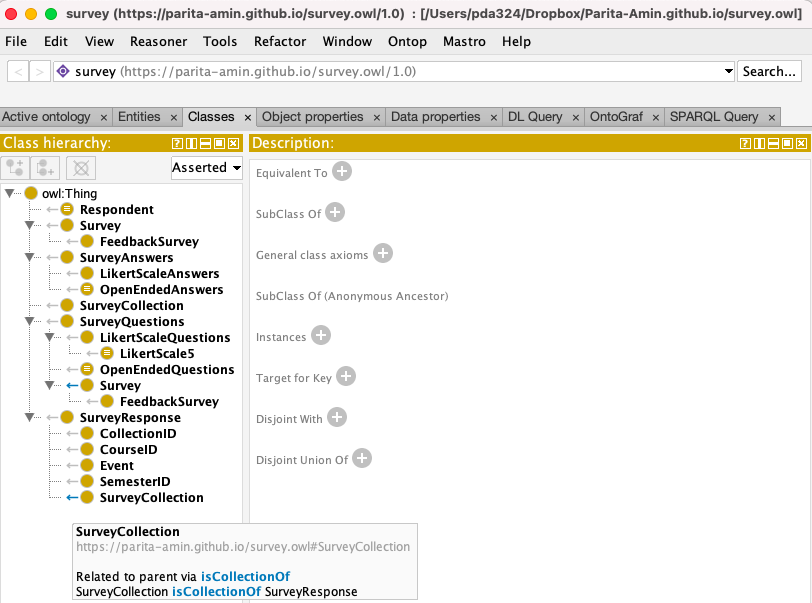
\includegraphics[width=15cm]{images/ch4/survey/final-survey-classes.png}
    \caption{Class Hierarchy for the Final Version of Survey Ontology}
    \label{final-survey-classes}
\end{figure}

The blue (\say{Survey} and \say{SurveyCollection} class) back arrow in front of the yellow solid dot, which indicates class, show parent/child relationship other than that of SubClassOf. This feature can be enabled and disabled by selecting \say{Display relationship in class hierarchy} option from the \say{View} menu of protégé. Figure~\ref{final-survey-classes} shows the relation indicated by the blue back arrow.

\subsection{Using SHACL for Data Validation}

\ac{shacl}4P is a protégé plugin for \ac{shacl}, which uses \say{shapes} to describe constraints. \ac{shacl} can be used to validate the manually entered data which are stored in spreadsheets. For feedback survey, the likert answers can only have values 1, 2, 3, 4, 5, or No Answer (blank cell). To restrict the values of data properties corresponding to likert questions in Figure~\ref{survey-data-properties}, \ac{shacl}4P has been used.

Protégé offers a view for \ac{shacl} editor as well as \ac{shacl} constraint violations. For successful working of \ac{shacl}4P, a reasoner should be enabled. The \ac{shacl} editor provides three buttons, namely, \say{Open}, \say{Save} , and \say{Validate}. After opening the shapes file (Open button), changes can be made and saved (Save button). Where as the Validate button allows users to validate the data. Figure~\ref{shacl-editor} shows a sample \say{SurveyShapes.txt} file opened in \ac{shacl} editor of protégé.

\begin{figure}[htp]
    \centering
    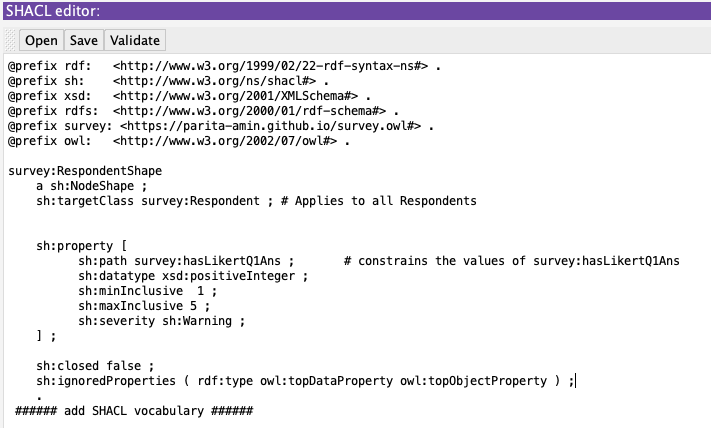
\includegraphics[width=15cm]{images/ch4/survey/shacl-editor.png}
    \caption{Data Validation using SHACL Editor}
    \label{shacl-editor}
\end{figure}

On clicking the Validate button, the summary of violated constraints is displayed on the \ac{shacl} constraint violations view in protégé. It contains the details like \say{Severity}, \say{SourceShape}, \say{Message}, \say{FocusNode}, \say{Path}, and \say{Value} as shown in Figure~\ref{shacl-constraint-violations}.

\begin{figure}[htp]
    \centering
    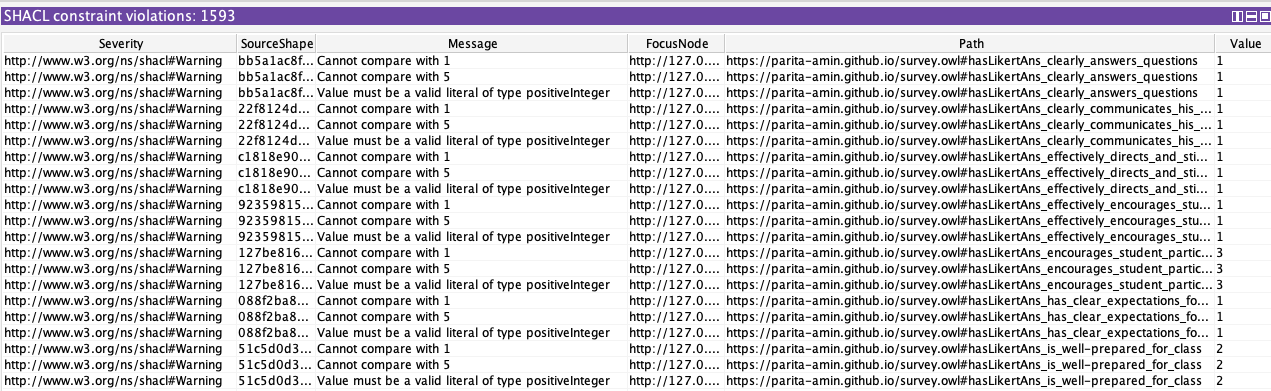
\includegraphics[width=15cm]{images/ch4/survey/shacl-constraint-violations.png}
    \caption{SHACL Constraint Violations}
    \label{shacl-constraint-violations}
\end{figure}

\subsection{Querying Survey Ontology in Protégé}

The ontology vocabularies can be queried using query languages like DL query and \ac{sparql}. A DL query is used to  such as `and' (corresponding to set intersection) and `some'.\footnote{https://ontology101tutorial.readthedocs.io/en/latest/EXERCISE\_BasicDL\_Queries.html}. \ac{sparql} query is used to express queries and optional graph patterns along with their conjunctions and disjunctions as well as aggregation, subqueries, negation, etc.\footnote{https://www.w3.org/TR/sparql11-query/} 

Protégé offers a plugin for DL as well as SPARQL queries. 

\subsubsection{DL Query}

\say{The DL Query tab allows users to quickly test definitions of classes to see that they subsume the appropriate subclasses. Or check for class membership of arbitrary descriptions without having to create named class placeholders.}\footnote{https://protegewiki.stanford.edu/wiki/DL\_Query} The DL Query tab can be opened using Tabs option under Windows menu. It is important to configure a reasoner to successfully express a DL query. Figure~\ref{survey-dl-query} shows expression of a sample DL query on the survey ontology in protégé. 

\begin{figure}[htp]
    \centering
    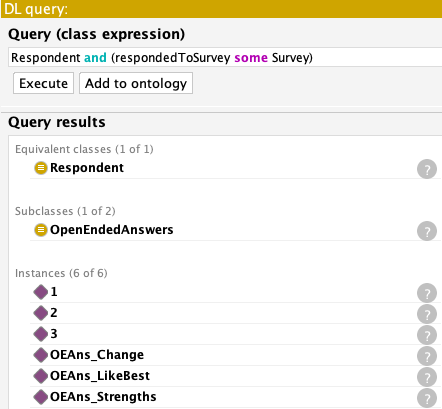
\includegraphics[width=15cm]{images/ch4/survey/survey-dl-query.png}
    \caption{DL Query on Survey Ontology}
    \label{survey-dl-query}
\end{figure}

\subsubsection{SPARQL Query}



\begin{figure}[htp]
    \centering
    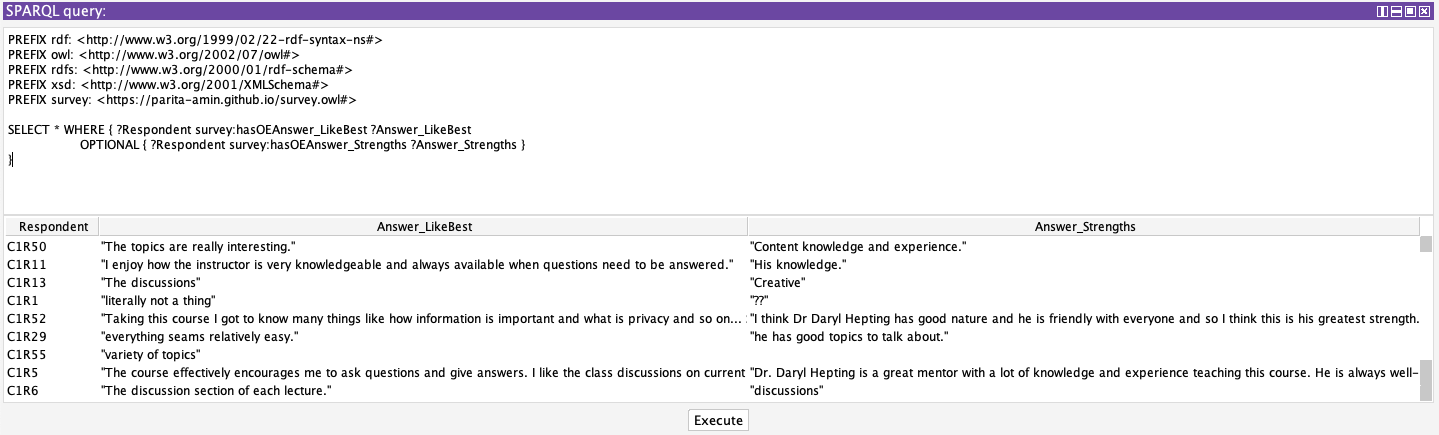
\includegraphics[width=15cm]{images/ch4/survey/survey-sparql-query.png}
    \caption{SPARQL Query on Survey Ontology}
    \label{survey-sparql-query}
\end{figure}

\begin{figure}[htp]
    \centering
    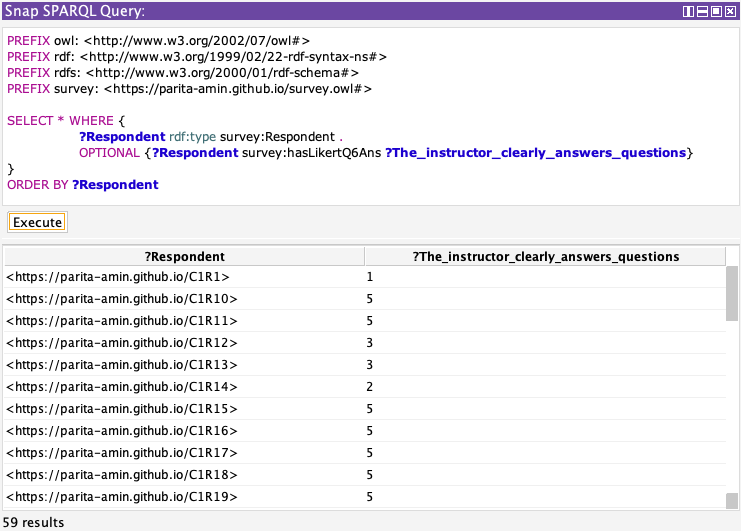
\includegraphics[width=15cm]{images/ch4/survey/survey-snap-sparql-query.png}
    \caption{Snap SPARQL Query on Survey Ontology}
    \label{survey-snap-sparql-query}
\end{figure}

\section{From Spreadsheets to Linked Open Data For Survey Ontology}

Primarily, OpenRefine\footnote{https://openrefine.org/} was used to convert the data stored in spreadsheets to Turtle and \ac{rdf} files.

\begin{figure}[htp]
    \centering
    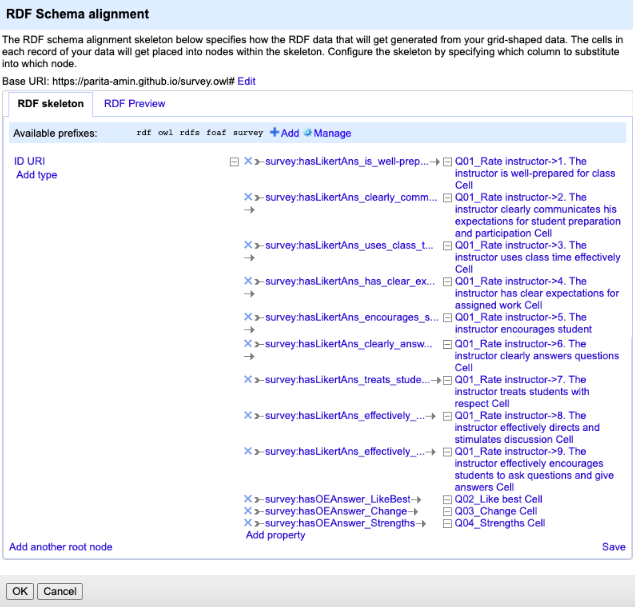
\includegraphics[width=15cm]{images/ch4/survey/survey-rdf-skeleton.png}
    \caption{RDF Skeleton for CSV using Survey Ontology}
    \label{survey-rdf-skeleton}
\end{figure}

\begin{figure}[htp]
    \centering
    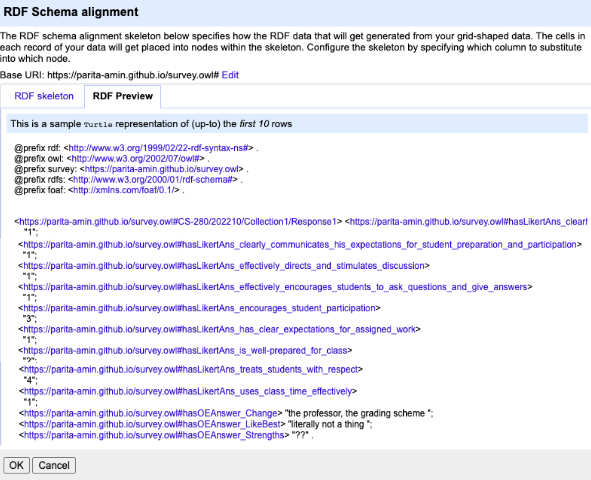
\includegraphics[width=15cm]{images/ch4/survey/survey-rdf-preview.png}
    \caption{RDF Preview for CSV using Survey Ontology}
    \label{survey-rdf-preview}
\end{figure}

\section{Licensing Survey Vocabulary}



\section{Publishing Linked Open Vocabulary for Survey}



\section{Visualization Tools for \ac{owl} Ontology}

The next step is visualization of the built \ac{owl} ontology using various visualization tools. Protégé supports plug-ins for some visualization tools like OntoGraf and \ac{owl}Viz whereas tools like WebVOWL, RelFinder and \ac{owl}GrEd are available for use as web-based tools. This section focuses on the two tools, OntoGraf and WebVOWL, used for the visualization of the survey ontology in this research.

\subsection{OntoGraf}

Falconer~\cite{falconer2010ontograf} introduced OntoGraf as a protégé plug-in for the visualization of the \ac{owl} ontologies. This tool helps the users to represent the ontologies, built using protégé, by repetitively allowing and restricting the desired classes. OntoGraf offers various graph layout options for visualization like Grid Layout\footnote{classes are arranged in a grid alphabetically}, Spring Layout, and Tree Layout\footnote{both horizontal and vertical}. Antoniazzi and Viola~\cite{antoniazz2018rdf} stated that the \say{individuals of a class can be visualized in its tooltip, but this is uncomfortable when dealing with a high number of assertional statements}. The graphs generated using OntoGraf can be exported as image files of various formats such as \ac{png}, \ac{jpeg}, \ac{gif} and as a dot file\footnote{a Microsoft Word Template with the details of default settings}.

Figure~\ref{ontograf} shows the graph generated using OntoGraf for the survey ontology. To start with the graph formation, the classes \say{Thing}, \say{Domain\_entity}, \say{Independent\_entity} and \say{Value} were selected followed by expansion of \say{Independent\_entity} and \say{Value} classes by double-clicking them. This expansion adds all the classes that are connected to the classes. The classes connected includes both the subclasses as well as the ones linked through the object properties. Solid blue lines are used to denote the relationships between the classes and their subclasses whereas dashed lines are used to represent the object properties.

\begin{figure}[htp]
    \centering
    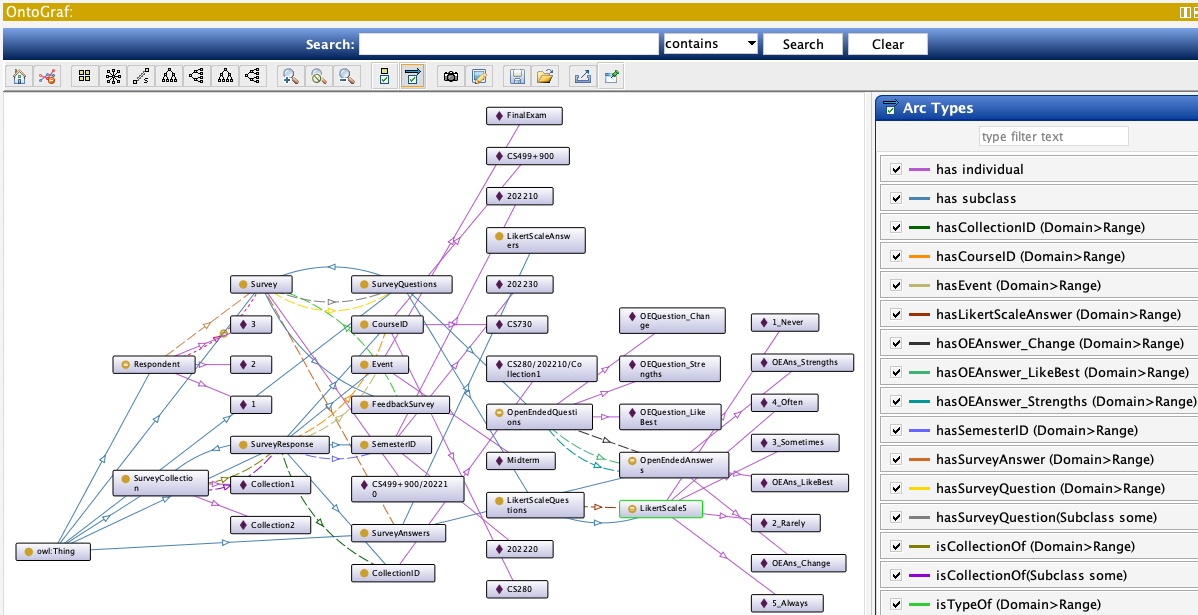
\includegraphics[width=15cm]{images/ch4/survey/ontograf.png}
    \caption{OntoGraf for Survey Ontology}
    \label{ontograf}
\end{figure}

\subsection{WebVOWL}

WebVOWL~\cite{lohmann2014webvowl}, the Web-based \ac{vowl}, one of the variety of forms in which the \ac{vowl} visualization tool is available, represents the \say{ontologies graphically using a force-directed graph layout}~\cite{antoniazz2018rdf}. \ac{vowl} follows some ground rules for the representation of \ac{owl} ontologies which are:

\begin{enumerate}
  
    \item Circles are used to denote classes. Also, different types are assigned different colors. For instance, \ac{owl} classes are denoted using \say{light blue circles}.

    \item Black solid lines are used to represent \ac{owl} object and datatype properties. The object properties use light blue labels where as the datatype properties are labelled in green.
  
    \item The relationships between the classes and their subclasses are represented using dashed lines.

\end{enumerate}

Figure~\ref{webVOWL} shows the graphical representation of the survey ontology using Web\ac{vowl}. The figure focuses on only some of the class-subclass relationships and some of the object properties. The metadata and the statistics of the node (circle) or the edge (line) can be retrieved by clicked on them. The entities (classes) and their relationships (object and datatype properties) can be presented or restricted using filters. The \ac{vowl} graph can be exported as an \ac{svg} image file or a \ac{json} code file.

\begin{figure}[htp]
    \centering
    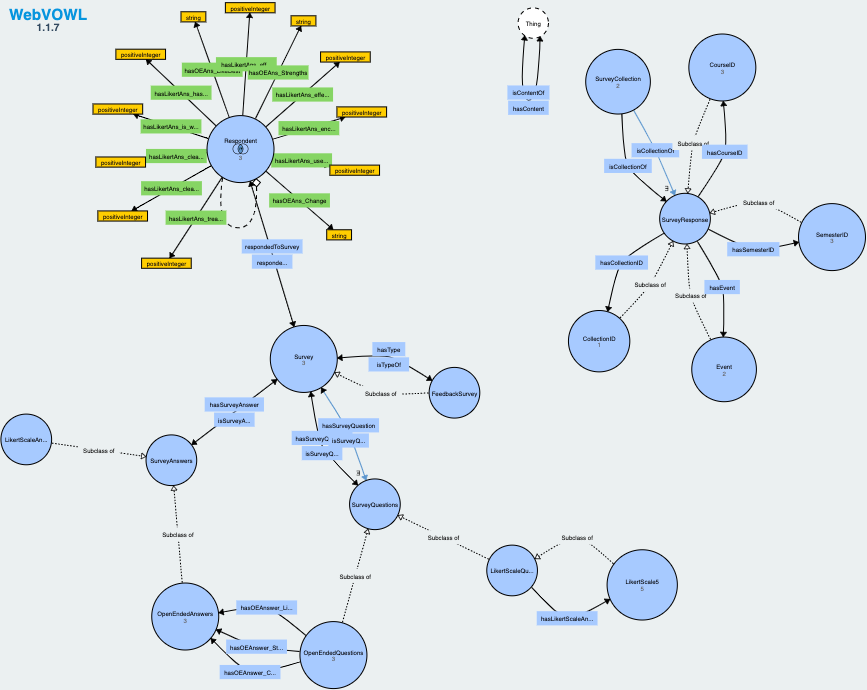
\includegraphics[width=15cm]{images/ch4/survey/webVOWL.png}
    \caption{WebVOWL for Survey Ontology}
    \label{webVOWL}
\end{figure}

\end{doublespace}
%!TEX root = parita-msc.tex

\chapter{Conclusion and Future Work}
\label{chap:conclusion}

\begin{doublespace}

%This Chapter focuses on the prime offerings of this research work where one of the sections includes the conclusions drawn from the work done and the other discusses future work that can be done to succeed in this research.

This Chapter presents a summary of the research undertaken and 
contained in this document.
It identifies the contributions made in this thesis and opportunities for future work.

\section{Conclusion}

After motivating the topic in Chapter 1,
Chapter 2 provides a detailed background study on the fundamental topics
supporting \ac{lod} and the tools which facilitate its publication on the web.
These include 
Semantic Web, 
Linked Open Data, 
\ac{rdf}, and 
\ac{owl} ontologies. 
This thesis describes the lifecycle of transforming data contained in a spreadsheet
into \ac{lod} that is available on the web of data, 
both in general terms (Chapter 3) 
and in the specific case of a student feedback survey (Chapter 4).
%a new attempt on developing a linked open data instrument for feedback surveys. 
%It focuses on the issues encountered and the user experience of various tools and references used for the modelling of the instrument and for data visualization. 
%The thesis revolves around some fundamental topics like 
%Semantic Web, 
%Linked Open Data, 
%\ac{rdf}, and 
%\ac{owl} ontologies. 
%It also describes how and why Protégé has been used over other ontology development tools to describe survey vocabularies. 
The thesis can be considered as a guide for researchers who are interested in 
transforming their own data into \ac{lod}.
%exploring this lesser known aspect of semantic web.

%the usability of protégé, and 
%discussion on some tools for linked open data visualizations. 
%Chapter~\ref{chap:methodology} describes the methodology followed to 
%describe, convert, visualize, and publish linked open data for survey in Chapter~\ref{chap:proofOfConcept}
%using protégé, OpenRefine, and the visual representation of the ontology 
%toward the end.

%thesis reviews the literature around publishing 

\section{Future Work}

Modelling of the range of Likert~\cite{what-is-Likert} scales.
with different labels and values.

Jekyll-RDF integration.

Conversion and management of all feedback data collected by Hepting

https://github.com/schimatos/schimatos.org -- data entry
Developing a data entry form for the feedback survey instrument
that can be defined in part ...


%This thesis also offers a number of future development options like building a real-time linked open data application for feedback surveys that 
%follows the linked data life cycle. 
%
%Web Scraping (or Web Extraction) 
%is a method of extracting desired data from the resources on the \ac{www} 
%into a separate file for data retrieval and data analysis. 
%Data Extraction is one of the steps in the linked data life cycle that can be explored in future research to facilitate use of data that has already been published to the web with \ac{html} tables.

Versioning of the survey ontology is a topic of interest. 
The ontology vocabularies can be reused for appropriate applications but they may need to be updated over time. 
Hence, 
ontology versioning and version management of the survey instrument for this feedback survey, 
as well as for other types of surveys is an aspect of this research that can be explored.

directly from the survey ontology would facilitate recording of survey responses collected offline.
\end{doublespace}

\addcontentsline{toc}{chapter}{References}
\bibliographystyle{plain}
\bibliography{thesis}

\appendix
%!TEX root = parita-msc.tex
\chapter{OWL Vocabulary for Survey Data: survey.owl}
\label{chap:appendix-owl}

OWL Vocabulary for Survey Data.
This is the OWL file that describes the feedback survey data received.

\UseRawInputEncoding
%\begin{doublespace}
\lstset{ 
  %backgroundcolor=\color{white},   % choose the background color; you must add \usepackage{color} or \usepackage{xcolor}; should come as last argument
  basicstyle=\footnotesize,        % the size of the fonts that are used for the code
  breakatwhitespace=true,         % sets if automatic breaks should only happen at whitespace
  breaklines=true,                 % sets automatic line breaking
  captionpos=b,                    % sets the caption-position to bottom
  %commentstyle=\color{mygreen},    % comment style
  %deletekeywords={...},            % if you want to delete keywords from the given language
  escapeinside={\%*}{*)},          % if you want to add LaTeX within your code
  %extendedchars=true,              % lets you use non-ASCII characters; for 8-bits encodings only, does not work with UTF-8
  firstnumber=1,                % start line enumeration with line 1000
  %frame=single,	                   % adds a frame around the code
  keepspaces=true,                 % keeps spaces in text, useful for keeping indentation of code (possibly needs columns=flexible)
  %keywordstyle=\color{blue},       % keyword style
  language=XML,                 % the language of the code
  %morekeywords={*,...},            % if you want to add more keywords to the set
  numbers=left,                    % where to put the line-numbers; possible values are (none, left, right)
  numbersep=5pt,                   % how far the line-numbers are from the code
  %numberstyle=\tiny\color{mygray}, % the style that is used for the line-numbers
  %rulecolor=\color{black},         % if not set, the frame-color may be changed on line-breaks within not-black text (e.g. comments (green here))
  showspaces=false,                % show spaces everywhere adding particular underscores; it overrides 'showstringspaces'
  showstringspaces=false,          % underline spaces within strings only
  showtabs=false,                  % show tabs within strings adding particular underscores
  stepnumber=1,                    % the step between two line-numbers. If it's 1, each line will be numbered
  %stringstyle=\color{mymauve},     % string literal style
  tabsize=2,	                   % sets default tabsize to 2 spaces
  title=\lstname                   % show the filename of files included with \lstinputlisting; also try caption instead of title
}
\begin{lstlisting}
@prefix : <https://parita-amin.github.io/survey.owl> .
@prefix owl: <http://www.w3.org/2002/07/owl#> .
@prefix rdf: <http://www.w3.org/1999/02/22-rdf-syntax-ns#> .
@prefix xml: <http://www.w3.org/XML/1998/namespace> .
@prefix xsd: <http://www.w3.org/2001/XMLSchema#> .
@prefix rdfs: <http://www.w3.org/2000/01/rdf-schema#> .
@prefix survey: <https://parita-amin.github.io/survey.owl#> .
@base <https://parita-amin.github.io/survey.owl> .

<https://parita-amin.github.io/survey.owl> rdf:type owl:Ontology ;
                                            owl:versionIRI <https://parita-amin.github.io/survey.owl/1.0> .

#################################################################
#    Object Properties
#################################################################

###  https://parita-amin.github.io/survey.owl#hasCollection
survey:hasCollection rdf:type owl:ObjectProperty ;
                     rdfs:domain survey:CourseOffering ;
                     rdfs:range survey:SurveyCollection .


###  https://parita-amin.github.io/survey.owl#hasCourseOffering
survey:hasCourseOffering rdf:type owl:ObjectProperty ;
                         rdfs:domain survey:HeptingStudentFeedbackSurvey ;
                         rdfs:range survey:CourseOffering .


###  https://parita-amin.github.io/survey.owl#hasEligibleRespondents
survey:hasEligibleRespondents rdf:type owl:ObjectProperty ;
                              rdfs:domain survey:SurveyCollection .


###  https://parita-amin.github.io/survey.owl#hasLikertScale
survey:hasLikertScale rdf:type owl:ObjectProperty ;
                      rdfs:domain survey:LikertQuestion ,
                                  survey:LikertScaleAnswer ;
                      rdfs:range survey:LikertScale .


###  https://parita-amin.github.io/survey.owl#hasQuestion
survey:hasQuestion rdf:type owl:ObjectProperty ;
                   rdfs:domain survey:Survey ;
                   rdfs:range survey:SurveyQuestion .


###  https://parita-amin.github.io/survey.owl#hasRespondent
survey:hasRespondent rdf:type owl:ObjectProperty ;
                     rdfs:domain survey:SurveyCollection ;
                     rdfs:range survey:SurveyRespondent .


###  https://parita-amin.github.io/survey.owl#isTypeOf
survey:isTypeOf rdf:type owl:ObjectProperty ;
                rdfs:domain survey:FeedbackSurvey ;
                rdfs:range survey:Survey .


#################################################################
#    Data properties
#################################################################

###  https://parita-amin.github.io/survey.owl#hasLSQ1Ans
survey:hasLSQ1Ans rdf:type owl:DatatypeProperty ;
                  rdfs:subPropertyOf owl:topDataProperty ;
                  rdfs:domain survey:LSQ1 ;
                  rdfs:range xsd:positiveInteger .


###  https://parita-amin.github.io/survey.owl#hasLSQ2Ans
survey:hasLSQ2Ans rdf:type owl:DatatypeProperty ;
                  rdfs:subPropertyOf owl:topDataProperty ;
                  rdfs:domain survey:LSQ2 ;
                  rdfs:range xsd:positiveInteger .


###  https://parita-amin.github.io/survey.owl#hasLSQ3Ans
survey:hasLSQ3Ans rdf:type owl:DatatypeProperty ;
                  rdfs:subPropertyOf owl:topDataProperty ;
                  rdfs:domain survey:LSQ3 ;
                  rdfs:range xsd:positiveInteger .


###  https://parita-amin.github.io/survey.owl#hasLSQ4Ans
survey:hasLSQ4Ans rdf:type owl:DatatypeProperty ;
                  rdfs:subPropertyOf owl:topDataProperty ;
                  rdfs:domain survey:LSQ4 ;
                  rdfs:range xsd:positiveInteger .


###  https://parita-amin.github.io/survey.owl#hasLSQ5Ans
survey:hasLSQ5Ans rdf:type owl:DatatypeProperty ;
                  rdfs:subPropertyOf owl:topDataProperty ;
                  rdfs:domain survey:LSQ5 ;
                  rdfs:range xsd:positiveInteger .


###  https://parita-amin.github.io/survey.owl#hasLSQ6Ans
survey:hasLSQ6Ans rdf:type owl:DatatypeProperty ;
                  rdfs:subPropertyOf owl:topDataProperty ;
                  rdfs:domain survey:LSQ6 ;
                  rdfs:range xsd:positiveInteger .


###  https://parita-amin.github.io/survey.owl#hasLSQ7Ans
survey:hasLSQ7Ans rdf:type owl:DatatypeProperty ;
                  rdfs:subPropertyOf owl:topDataProperty ;
                  rdfs:domain survey:LSQ7 ;
                  rdfs:range xsd:positiveInteger .


###  https://parita-amin.github.io/survey.owl#hasLSQ8Ans
survey:hasLSQ8Ans rdf:type owl:DatatypeProperty ;
                  rdfs:subPropertyOf owl:topDataProperty ;
                  rdfs:domain survey:LSQ8 ;
                  rdfs:range xsd:positiveInteger .


###  https://parita-amin.github.io/survey.owl#hasLSQ9Ans
survey:hasLSQ9Ans rdf:type owl:DatatypeProperty ;
                  rdfs:subPropertyOf owl:topDataProperty ;
                  rdfs:domain survey:LSQ9 ;
                  rdfs:range xsd:positiveInteger .


###  https://parita-amin.github.io/survey.owl#hasOEQ1Ans
survey:hasOEQ1Ans rdf:type owl:DatatypeProperty ;
                  rdfs:subPropertyOf owl:topDataProperty ;
                  rdfs:domain survey:OEQ1 ;
                  rdfs:range xsd:string .


###  https://parita-amin.github.io/survey.owl#hasOEQ2Ans
survey:hasOEQ2Ans rdf:type owl:DatatypeProperty ;
                  rdfs:subPropertyOf owl:topDataProperty ;
                  rdfs:domain survey:OEQ2 ;
                  rdfs:range xsd:string .


###  https://parita-amin.github.io/survey.owl#hasOEQ3Ans
survey:hasOEQ3Ans rdf:type owl:DatatypeProperty ;
                  rdfs:subPropertyOf owl:topDataProperty ;
                  rdfs:domain survey:OEQ3 ;
                  rdfs:range xsd:string .


###  https://parita-amin.github.io/survey.owl#hasQuestionText
survey:hasQuestionText rdf:type owl:DatatypeProperty ;
                       rdfs:domain survey:SurveyQuestion ;
                       rdfs:range xsd:string .


#################################################################
#    Classes
#################################################################

###  https://parita-amin.github.io/survey.owl#CourseOffering
survey:CourseOffering rdf:type owl:Class ;
                      rdfs:subClassOf survey:SurveyCollection ,
                                      [ rdf:type owl:Restriction ;
                                        owl:onProperty survey:hasCollection ;
                                        owl:someValuesFrom survey:SurveyCollection
                                      ] .


###  https://parita-amin.github.io/survey.owl#FeedbackSurvey
survey:FeedbackSurvey rdf:type owl:Class ;
                      rdfs:subClassOf survey:Survey ;
                      owl:disjointWith survey:FeedbackSurveyRespondent .


###  https://parita-amin.github.io/survey.owl#FeedbackSurveyRespondent
survey:FeedbackSurveyRespondent rdf:type owl:Class ;
                                rdfs:subClassOf survey:SurveyRespondent .


###  https://parita-amin.github.io/survey.owl#HeptingStudentFeedbackSurvey
survey:HeptingStudentFeedbackSurvey rdf:type owl:Class ;
                                    rdfs:subClassOf survey:FeedbackSurvey ;
                                    owl:disjointWith survey:HeptingStudentFeedbackSurveyRespondent .


###  https://parita-amin.github.io/survey.owl#HeptingStudentFeedbackSurveyRespondent
survey:HeptingStudentFeedbackSurveyRespondent rdf:type owl:Class ;
                                              rdfs:subClassOf survey:FeedbackSurveyRespondent .


###  https://parita-amin.github.io/survey.owl#LSQ1
survey:LSQ1 rdf:type owl:Class ;
            rdfs:subClassOf survey:LikertQuestion ,
                            [ rdf:type owl:Restriction ;
                              owl:onProperty survey:hasQuestionText ;
                              owl:hasValue "The instructor is well-prepared for class"
                            ] .


###  https://parita-amin.github.io/survey.owl#LSQ1Ans
survey:LSQ1Ans rdf:type owl:Class ;
               rdfs:subClassOf survey:LikertScaleAnswer .


###  https://parita-amin.github.io/survey.owl#LSQ2
survey:LSQ2 rdf:type owl:Class ;
            rdfs:subClassOf survey:LikertQuestion ,
                            [ rdf:type owl:Restriction ;
                              owl:onProperty survey:hasQuestionText ;
                              owl:hasValue "The instructor clearly communicates his expectations for student preparation and participation"
                            ] .


###  https://parita-amin.github.io/survey.owl#LSQ2Ans
survey:LSQ2Ans rdf:type owl:Class ;
               rdfs:subClassOf survey:LikertScaleAnswer .


###  https://parita-amin.github.io/survey.owl#LSQ3
survey:LSQ3 rdf:type owl:Class ;
            rdfs:subClassOf survey:LikertQuestion ,
                            [ rdf:type owl:Restriction ;
                              owl:onProperty survey:hasQuestionText ;
                              owl:hasValue "The instructor uses class time effectively"
                            ] .


###  https://parita-amin.github.io/survey.owl#LSQ3Ans
survey:LSQ3Ans rdf:type owl:Class ;
               rdfs:subClassOf survey:LikertScaleAnswer .


###  https://parita-amin.github.io/survey.owl#LSQ4
survey:LSQ4 rdf:type owl:Class ;
            rdfs:subClassOf survey:LikertQuestion ,
                            [ rdf:type owl:Restriction ;
                              owl:onProperty survey:hasQuestionText ;
                              owl:hasValue "The instructor has clear expectations for assigned work"
                            ] .


###  https://parita-amin.github.io/survey.owl#LSQ4Ans
survey:LSQ4Ans rdf:type owl:Class ;
               rdfs:subClassOf survey:LikertScaleAnswer .


###  https://parita-amin.github.io/survey.owl#LSQ5
survey:LSQ5 rdf:type owl:Class ;
            rdfs:subClassOf survey:LikertQuestion ,
                            [ rdf:type owl:Restriction ;
                              owl:onProperty survey:hasQuestionText ;
                              owl:hasValue "The instructor encourages student participation"
                            ] .


###  https://parita-amin.github.io/survey.owl#LSQ5Ans
survey:LSQ5Ans rdf:type owl:Class ;
               rdfs:subClassOf survey:LikertScaleAnswer .


###  https://parita-amin.github.io/survey.owl#LSQ6
survey:LSQ6 rdf:type owl:Class ;
            rdfs:subClassOf survey:LikertQuestion ,
                            [ rdf:type owl:Restriction ;
                              owl:onProperty survey:hasQuestionText ;
                              owl:hasValue "The instructor clearly answers questions"
                            ] .


###  https://parita-amin.github.io/survey.owl#LSQ6Ans
survey:LSQ6Ans rdf:type owl:Class ;
               rdfs:subClassOf survey:LikertScaleAnswer .


###  https://parita-amin.github.io/survey.owl#LSQ7
survey:LSQ7 rdf:type owl:Class ;
            rdfs:subClassOf survey:LikertQuestion ,
                            [ rdf:type owl:Restriction ;
                              owl:onProperty survey:hasQuestionText ;
                              owl:hasValue "The instructor treats students with respect"
                            ] .


###  https://parita-amin.github.io/survey.owl#LSQ7Ans
survey:LSQ7Ans rdf:type owl:Class ;
               rdfs:subClassOf survey:LikertScaleAnswer .


###  https://parita-amin.github.io/survey.owl#LSQ8
survey:LSQ8 rdf:type owl:Class ;
            rdfs:subClassOf survey:LikertQuestion ,
                            [ rdf:type owl:Restriction ;
                              owl:onProperty survey:hasQuestionText ;
                              owl:hasValue "The instructor effectively directs and stimulates discussion"
                            ] .


###  https://parita-amin.github.io/survey.owl#LSQ8Ans
survey:LSQ8Ans rdf:type owl:Class ;
               rdfs:subClassOf survey:LikertScaleAnswer .


###  https://parita-amin.github.io/survey.owl#LSQ9
survey:LSQ9 rdf:type owl:Class ;
            rdfs:subClassOf survey:LikertQuestion ,
                            [ rdf:type owl:Restriction ;
                              owl:onProperty survey:hasQuestionText ;
                              owl:hasValue "The instructor effectively encourages students to ask questions and give answers"
                            ] .


###  https://parita-amin.github.io/survey.owl#LSQ9Ans
survey:LSQ9Ans rdf:type owl:Class ;
               rdfs:subClassOf survey:LikertScaleAnswer .


###  https://parita-amin.github.io/survey.owl#LikertQuestion
survey:LikertQuestion rdf:type owl:Class ;
                      rdfs:subClassOf survey:LikertScaleQuestion ,
                                      [ rdf:type owl:Restriction ;
                                        owl:onProperty survey:hasLikertScale ;
                                        owl:someValuesFrom survey:LikertScale
                                      ] .


###  https://parita-amin.github.io/survey.owl#LikertScale
survey:LikertScale rdf:type owl:Class ;
                   owl:equivalentClass [ rdf:type owl:Class ;
                                         owl:oneOf ( <https://parita-amin.github.io/survey.owl#1>
                                                     <https://parita-amin.github.io/survey.owl#2>
                                                     <https://parita-amin.github.io/survey.owl#3>
                                                     <https://parita-amin.github.io/survey.owl#4>
                                                     <https://parita-amin.github.io/survey.owl#5>
                                                   )
                                       ] ;
                   rdfs:subClassOf survey:LikertScaleQuestion .


###  https://parita-amin.github.io/survey.owl#LikertScaleAnswer
survey:LikertScaleAnswer rdf:type owl:Class ;
                         rdfs:subClassOf survey:SurveyAnswer ,
                                         [ rdf:type owl:Restriction ;
                                           owl:onProperty survey:hasLikertScale ;
                                           owl:someValuesFrom survey:LikertScale
                                         ] ;
                         owl:disjointWith survey:OpenEndedAnswer .


###  https://parita-amin.github.io/survey.owl#LikertScaleQuestion
survey:LikertScaleQuestion rdf:type owl:Class ;
                           rdfs:subClassOf survey:SurveyQuestion ,
                                           [ rdf:type owl:Restriction ;
                                             owl:onProperty survey:hasLikertScale ;
                                             owl:qualifiedCardinality "1"^^xsd:nonNegativeInteger ;
                                             owl:onClass survey:LikertScale
                                           ] ;
                           owl:disjointWith survey:OpenEndedQuestion .


###  https://parita-amin.github.io/survey.owl#OEQ1
survey:OEQ1 rdf:type owl:Class ;
            rdfs:subClassOf survey:OpenEndedQuestion ,
                            [ rdf:type owl:Restriction ;
                              owl:onProperty survey:hasQuestionText ;
                              owl:hasValue "What do you like best about the course?"
                            ] .


###  https://parita-amin.github.io/survey.owl#OEQ1Ans
survey:OEQ1Ans rdf:type owl:Class ;
               rdfs:subClassOf survey:OpenEndedAnswer ,
                               [ rdf:type owl:Restriction ;
                                 owl:onProperty survey:hasOEQ1Ans ;
                                 owl:someValuesFrom xsd:string
                               ] .


###  https://parita-amin.github.io/survey.owl#OEQ2
survey:OEQ2 rdf:type owl:Class ;
            rdfs:subClassOf survey:OpenEndedQuestion ,
                            [ rdf:type owl:Restriction ;
                              owl:onProperty survey:hasQuestionText ;
                              owl:hasValue "What would you like to change about the course?"
                            ] .


###  https://parita-amin.github.io/survey.owl#OEQ2Ans
survey:OEQ2Ans rdf:type owl:Class ;
               rdfs:subClassOf survey:OpenEndedAnswer ,
                               [ rdf:type owl:Restriction ;
                                 owl:onProperty survey:hasOEQ2Ans ;
                                 owl:someValuesFrom xsd:string
                               ] .


###  https://parita-amin.github.io/survey.owl#OEQ3
survey:OEQ3 rdf:type owl:Class ;
            rdfs:subClassOf survey:OpenEndedQuestion ,
                            [ rdf:type owl:Restriction ;
                              owl:onProperty survey:hasQuestionText ;
                              owl:hasValue "What do you think the instructor's greatest strengths are?"
                            ] .


###  https://parita-amin.github.io/survey.owl#OEQ3Ans
survey:OEQ3Ans rdf:type owl:Class ;
               rdfs:subClassOf survey:OpenEndedAnswer ,
                               [ rdf:type owl:Restriction ;
                                 owl:onProperty survey:hasOEQ3Ans ;
                                 owl:someValuesFrom xsd:string
                               ] .


###  https://parita-amin.github.io/survey.owl#OpenEndedAnswer
survey:OpenEndedAnswer rdf:type owl:Class ;
                       rdfs:subClassOf survey:SurveyAnswer .


###  https://parita-amin.github.io/survey.owl#OpenEndedQuestion
survey:OpenEndedQuestion rdf:type owl:Class ;
                         rdfs:subClassOf survey:SurveyQuestion .


###  https://parita-amin.github.io/survey.owl#Survey
survey:Survey rdf:type owl:Class ;
              rdfs:subClassOf [ rdf:type owl:Restriction ;
                                owl:onProperty survey:hasQuestion ;
                                owl:someValuesFrom survey:SurveyQuestion
                              ] .


###  https://parita-amin.github.io/survey.owl#SurveyAnswer
survey:SurveyAnswer rdf:type owl:Class ;
                    rdfs:subClassOf survey:HeptingStudentFeedbackSurveyRespondent .


###  https://parita-amin.github.io/survey.owl#SurveyCollection
survey:SurveyCollection rdf:type owl:Class ;
                        rdfs:subClassOf [ rdf:type owl:Restriction ;
                                          owl:onProperty survey:hasEligibleRespondents ;
                                          owl:someValuesFrom survey:SurveyRespondent
                                        ] .


###  https://parita-amin.github.io/survey.owl#SurveyQuestion
survey:SurveyQuestion rdf:type owl:Class ;
                      rdfs:subClassOf survey:HeptingStudentFeedbackSurvey ,
                                      [ rdf:type owl:Restriction ;
                                        owl:onProperty survey:hasQuestionText ;
                                        owl:qualifiedCardinality "1"^^xsd:nonNegativeInteger ;
                                        owl:onDataRange xsd:string
                                      ] .


###  https://parita-amin.github.io/survey.owl#SurveyRespondent
survey:SurveyRespondent rdf:type owl:Class ;
                        rdfs:subClassOf [ rdf:type owl:Restriction ;
                                          owl:onProperty survey:hasCollection ;
                                          owl:someValuesFrom survey:SurveyCollection
                                        ] .


#################################################################
#    Individuals
#################################################################

###  https://parita-amin.github.io/survey.owl#1
<https://parita-amin.github.io/survey.owl#1> rdf:type owl:NamedIndividual ,
                                                      survey:LikertScale .


###  https://parita-amin.github.io/survey.owl#2
<https://parita-amin.github.io/survey.owl#2> rdf:type owl:NamedIndividual ,
                                                      survey:LikertScale .


###  https://parita-amin.github.io/survey.owl#3
<https://parita-amin.github.io/survey.owl#3> rdf:type owl:NamedIndividual ,
                                                      survey:LikertScale .


###  https://parita-amin.github.io/survey.owl#4
<https://parita-amin.github.io/survey.owl#4> rdf:type owl:NamedIndividual ,
                                                      survey:LikertScale .


###  https://parita-amin.github.io/survey.owl#5
<https://parita-amin.github.io/survey.owl#5> rdf:type owl:NamedIndividual ,
                                                      survey:LikertScale .


#################################################################
#    General axioms
#################################################################

[ rdf:type owl:AllDisjointClasses ;
  owl:members ( survey:LSQ1
                survey:LSQ2
                survey:LSQ3
              )
] .


[ rdf:type owl:AllDisjointClasses ;
  owl:members ( survey:LSQ1
                survey:LSQ2
                survey:LSQ3
                survey:LSQ4
                survey:LSQ5
                survey:LSQ6
                survey:LSQ7
                survey:LSQ8
                survey:LSQ9
              )
] .


[ rdf:type owl:AllDisjointClasses ;
  owl:members ( survey:LSQ1Ans
                survey:LSQ2Ans
                survey:LSQ3Ans
                survey:LSQ4Ans
                survey:LSQ5Ans
                survey:LSQ6Ans
                survey:LSQ7Ans
                survey:LSQ8Ans
                survey:LSQ9Ans
              )
] .


[ rdf:type owl:AllDisjointClasses ;
  owl:members ( survey:OEQ1
                survey:OEQ2
                survey:OEQ3
              )
] .


[ rdf:type owl:AllDisjointClasses ;
  owl:members ( survey:Survey
                survey:SurveyCollection
                survey:SurveyRespondent
              )
] .


###  Generated by the OWL API (version 4.5.9.2019-02-01T07:24:44Z) https://github.com/owlcs/owlapi

\end{lstlisting}
%\end{doublespace}

\chapter{CSV to Linked Data: sample.ttl}
\label{chap:appendix-data}

\UseRawInputEncoding
%\begin{doublespace}
\lstset{ 
  %backgroundcolor=\color{white},   % choose the background color; you must add \usepackage{color} or \usepackage{xcolor}; should come as last argument
  basicstyle=\footnotesize,        % the size of the fonts that are used for the code
  breakatwhitespace=true,         % sets if automatic breaks should only happen at whitespace
  breaklines=true,                 % sets automatic line breaking
  captionpos=b,                    % sets the caption-position to bottom
  %commentstyle=\color{mygreen},    % comment style
  %deletekeywords={...},            % if you want to delete keywords from the given language
  escapeinside={\%*}{*)},          % if you want to add LaTeX within your code
  %extendedchars=true,              % lets you use non-ASCII characters; for 8-bits encodings only, does not work with UTF-8
  firstnumber=1,                % start line enumeration with line 1000
  %frame=single,	                   % adds a frame around the code
  keepspaces=true,                 % keeps spaces in text, useful for keeping indentation of code (possibly needs columns=flexible)
  %keywordstyle=\color{blue},       % keyword style
  language=XML,                 % the language of the code
  %morekeywords={*,...},            % if you want to add more keywords to the set
  numbers=left,                    % where to put the line-numbers; possible values are (none, left, right)
  numbersep=5pt,                   % how far the line-numbers are from the code
  %numberstyle=\tiny\color{mygray}, % the style that is used for the line-numbers
  %rulecolor=\color{black},         % if not set, the frame-color may be changed on line-breaks within not-black text (e.g. comments (green here))
  showspaces=false,                % show spaces everywhere adding particular underscores; it overrides 'showstringspaces'
  showstringspaces=false,          % underline spaces within strings only
  showtabs=false,                  % show tabs within strings adding particular underscores
  stepnumber=1,                    % the step between two line-numbers. If it's 1, each line will be numbered
  %stringstyle=\color{mymauve},     % string literal style
  tabsize=2,	                   % sets default tabsize to 2 spaces
  title=\lstname                   % show the filename of files included with \lstinputlisting; also try caption instead of title
}
\begin{lstlisting}
@prefix rdf: <http://www.w3.org/1999/02/22-rdf-syntax-ns#> .
@prefix owl: <http://www.w3.org/2002/07/owl#> .
@prefix xsd: <http://www.w3.org/2001/XMLSchema#> .
@prefix survey: <https://parita-amin.github.io/survey.owl#> .
@prefix rdfs: <http://www.w3.org/2000/01/rdf-schema#> .
@prefix foaf: <http://xmlns.com/foaf/0.1/> .
@prefix : <https://parita-amin.github.io/survey.owl/> .

:CS-280-202210 a survey:Course;
	survey:hasCollection :Collection1.

:Collection1 a survey:SurveyCollection;
  	survey:hasEligibleRespondents "100"^^xsd:int;
  	survey:hasRespondent
		:C1R1,
		:C1R2,
		:C1R3,
		:C1R4,
		:C1R5,
		:C1R6,
		:C1R7,
		:C1R8,
		:C1R9,
		:C1R10,
		:C1R11,
		:C1R12,
		:C1R13,
		:C1R14,
		:C1R15,
		:C1R16,
		:C1R17,
		:C1R18,
		:C1R19,
		:C1R20,
		:C1R21,
		:C1R22,
		:C1R23,
		:C1R24,
		:C1R25,
		:C1R26,
		:C1R27,
		:C1R28,
		:C1R29,
		:C1R30,
		:C1R31,
		:C1R32,
		:C1R33,
		:C1R34,
		:C1R35,
		:C1R36,
		:C1R37,
		:C1R38,
		:C1R39,
		:C1R40,
		:C1R41,
		:C1R42,
		:C1R43,
		:C1R44,
		:C1R45,
		:C1R46,
		:C1R47,
		:C1R48,
		:C1R49,
		:C1R50,
		:C1R51,
		:C1R52,
		:C1R53,
		:C1R54,
		:C1R55,
		:C1R56,
		:C1R57,
		:C1R58,
		:C1R59.

:C1R1 a survey:Respondent;
	survey:hasLikertQ6Ans "1"^^xsd:positiveInteger;
	survey:hasLikertQ2Ans "1"^^xsd:positiveInteger;
	survey:hasLikertQ8Ans "1"^^xsd:positiveInteger;
	survey:hasLikertQ9Ans "1"^^xsd:positiveInteger;
	survey:hasLikertQ5Ans "3"^^xsd:positiveInteger;
	survey:hasLikertQ4Ans "1"^^xsd:positiveInteger;
	survey:hasLikertQ1Ans "2"^^xsd:positiveInteger;
	survey:hasLikertQ7Ans "4"^^xsd:positiveInteger;
	survey:hasLikertQ3Ans "1"^^xsd:positiveInteger;
	survey:hasOEAnswer_Change "the professor, the grading scheme";
	survey:hasOEAnswer_LikeBest "literally not a thing";
	survey:hasOEAnswer_Strengths "??" .

:C1R2 a survey:Respondent;
	survey:hasLikertQ6Ans "5"^^xsd:positiveInteger;
	survey:hasLikertQ2Ans "5"^^xsd:positiveInteger;
	survey:hasLikertQ8Ans "4"^^xsd:positiveInteger;
	survey:hasLikertQ9Ans "4"^^xsd:positiveInteger;
	survey:hasLikertQ5Ans "5"^^xsd:positiveInteger;
	survey:hasLikertQ4Ans "5"^^xsd:positiveInteger;
	survey:hasLikertQ1Ans "4"^^xsd:positiveInteger;
	survey:hasLikertQ7Ans "5"^^xsd:positiveInteger;
	survey:hasLikertQ3Ans "2"^^xsd:positiveInteger;
	survey:hasOEAnswer_Change "I feel like if we had some more information about debate topics we would be able to debate more effectively.";
	survey:hasOEAnswer_LikeBest "I like how quick the teacher is to answer any question about a assignment or a project and clarify any detail.";
	survey:hasOEAnswer_Strengths "The teacher always answers questions about assignments and projects when ever he is asked about them so I always feel prepared for the next assignment." .

:C1R3 a survey:Respondent;
	survey:hasLikertQ6Ans "4"^^xsd:positiveInteger;
	survey:hasLikertQ2Ans "4"^^xsd:positiveInteger;
	survey:hasLikertQ8Ans "4"^^xsd:positiveInteger;
  	survey:hasLikertQ9Ans "4"^^xsd:positiveInteger;
  	survey:hasLikertQ5Ans "4"^^xsd:positiveInteger;
  	survey:hasLikertQ4Ans "4"^^xsd:positiveInteger;
  	survey:hasLikertQ1Ans "4"^^xsd:positiveInteger;
  	survey:hasLikertQ7Ans "4"^^xsd:positiveInteger;
  	survey:hasLikertQ3Ans "4"^^xsd:positiveInteger .

:C1R4 a survey:Respondent;
 	survey:hasLikertQ6Ans "3"^^xsd:positiveInteger;
  	survey:hasLikertQ2Ans "4"^^xsd:positiveInteger;
  	survey:hasLikertQ8Ans "4"^^xsd:positiveInteger;
  	survey:hasLikertQ9Ans "5"^^xsd:positiveInteger;
  	survey:hasLikertQ5Ans "5"^^xsd:positiveInteger;
  	survey:hasLikertQ4Ans "2"^^xsd:positiveInteger;
  	survey:hasLikertQ1Ans "3"^^xsd:positiveInteger;
  	survey:hasLikertQ7Ans "5"^^xsd:positiveInteger;
  	survey:hasLikertQ3Ans "3"^^xsd:positiveInteger;
  	survey:hasOEAnswer_Change "I am confused on what the topics of this course even are. Every class it's students asking questions about the assignments and projects and then we have about 15 minutes at the end of every class to try and have a discussion.";
	survey:hasOEAnswer_Strengths "Having open communication with the students. No one is afraid to turn their microphones on and talk or share an opinion. It is a very welcoming environment." .

:C1R5 a survey:Respondent;
	survey:hasLikertQ6Ans "5"^^xsd:positiveInteger;
  	survey:hasLikertQ2Ans "5"^^xsd:positiveInteger;
  	survey:hasLikertQ8Ans "5"^^xsd:positiveInteger;
  	survey:hasLikertQ9Ans "5"^^xsd:positiveInteger;
  	survey:hasLikertQ5Ans "5"^^xsd:positiveInteger;
  	survey:hasLikertQ4Ans "5"^^xsd:positiveInteger;
  	survey:hasLikertQ1Ans "5"^^xsd:positiveInteger;
  	survey:hasLikertQ7Ans "5"^^xsd:positiveInteger;
  	survey:hasLikertQ3Ans "4"^^xsd:positiveInteger;
  	survey:hasOEAnswer_Change "This class is different from all the other classes I have taken. The discussions are open-ended and sometimes I feel I am not sure how well I am doing in this class or what I am learning. I would like to see more concrete implementation for achieving the desired learning outcomes. I do not what would be there on the final exam and what should I need to do to pass the final exam.";
  	survey:hasOEAnswer_LikeBest "The course effectively encourages me to ask questions and give answers. I like the class discussions on current topics in the world, helps me keep myself aware of what is happening in the world.";
  	survey:hasOEAnswer_Strengths "Dr. Daryl Hepting is a great mentor with a lot of knowledge and experience teaching this course. He is always well-prepared for the class and communicates his expectations for students clearly. His teaching style encourages student participation. He is very respectful of his students and always willing to go above and beyond for helping his students. I would definitely take another class with Dr. Hepting." .

:C1R6 a survey:Respondent;
	survey:hasLikertQ6Ans "3"^^xsd:positiveInteger;
  	survey:hasLikertQ2Ans "2"^^xsd:positiveInteger;
  	survey:hasLikertQ8Ans "4"^^xsd:positiveInteger;
  	survey:hasLikertQ9Ans "5"^^xsd:positiveInteger;
  	survey:hasLikertQ5Ans "5"^^xsd:positiveInteger;
  	survey:hasLikertQ4Ans "2"^^xsd:positiveInteger;
  	survey:hasLikertQ1Ans "2"^^xsd:positiveInteger;
  	survey:hasLikertQ7Ans "5"^^xsd:positiveInteger;
  	survey:hasLikertQ3Ans "1"^^xsd:positiveInteger;
  	survey:hasOEAnswer_Change "The clarity on what is expected of us on assignments.";
  	survey:hasOEAnswer_LikeBest "The discussion section of each lecture.";
  	survey:hasOEAnswer_Strengths "discussions" .

:C1R7 a survey:Respondent;
	survey:hasLikertQ6Ans "1"^^xsd:positiveInteger;
  	survey:hasLikertQ2Ans "1"^^xsd:positiveInteger;
  	survey:hasLikertQ8Ans "2"^^xsd:positiveInteger;
  	survey:hasLikertQ9Ans "2"^^xsd:positiveInteger;
  	survey:hasLikertQ5Ans "3"^^xsd:positiveInteger;
  	survey:hasLikertQ4Ans "2"^^xsd:positiveInteger;
  	survey:hasLikertQ1Ans "1"^^xsd:positiveInteger;
  	survey:hasLikertQ7Ans "3"^^xsd:positiveInteger;
  	survey:hasLikertQ3Ans "1"^^xsd:positiveInteger .

:C1R8 a survey:Respondent;
	survey:hasLikertQ6Ans "3"^^xsd:positiveInteger;
  	survey:hasLikertQ2Ans "3"^^xsd:positiveInteger;
  	survey:hasLikertQ8Ans "3"^^xsd:positiveInteger;
  	survey:hasLikertQ9Ans "3"^^xsd:positiveInteger;
  	survey:hasLikertQ5Ans "3"^^xsd:positiveInteger;
  	survey:hasLikertQ4Ans "3"^^xsd:positiveInteger;
  	survey:hasLikertQ1Ans "3"^^xsd:positiveInteger;
  	survey:hasLikertQ7Ans "3"^^xsd:positiveInteger;
  	survey:hasLikertQ3Ans "3"^^xsd:positiveInteger;
  	survey:hasOEAnswer_Change "Nothing";
  	survey:hasOEAnswer_LikeBest "The content";
  	survey:hasOEAnswer_Strengths "His communication skills" .

:C1R9 a survey:Respondent;
	survey:hasLikertQ6Ans "4"^^xsd:positiveInteger;
  	survey:hasLikertQ2Ans "3"^^xsd:positiveInteger;
  	survey:hasLikertQ8Ans "5"^^xsd:positiveInteger;
  	survey:hasLikertQ9Ans "5"^^xsd:positiveInteger;
  	survey:hasLikertQ5Ans "5"^^xsd:positiveInteger;
  	survey:hasLikertQ4Ans "4"^^xsd:positiveInteger;
  	survey:hasLikertQ1Ans "3"^^xsd:positiveInteger;
  	survey:hasLikertQ7Ans "5"^^xsd:positiveInteger;
  	survey:hasLikertQ3Ans "4"^^xsd:positiveInteger .

:C1R10 a survey:Respondent;
		  survey:hasLikertQ6Ans "5"^^xsd:positiveInteger;
		  survey:hasLikertQ2Ans "5"^^xsd:positiveInteger;
		  survey:hasLikertQ8Ans "5"^^xsd:positiveInteger;
		  survey:hasLikertQ9Ans "5"^^xsd:positiveInteger;
		  survey:hasLikertQ5Ans "5"^^xsd:positiveInteger;
		  survey:hasLikertQ4Ans "5"^^xsd:positiveInteger;
		  survey:hasLikertQ1Ans "5"^^xsd:positiveInteger;
		  survey:hasLikertQ7Ans "5"^^xsd:positiveInteger;
		  survey:hasLikertQ3Ans "5"^^xsd:positiveInteger;
		  survey:hasOEAnswer_Change "NO";
		  survey:hasOEAnswer_LikeBest "The teacher's lessons are very informative, and then you need to reply every day so that people can discuss the content of the daily lessons.";
		  survey:hasOEAnswer_Strengths "NO" .

:C1R11 a survey:Respondent;
		  survey:hasLikertQ6Ans "5"^^xsd:positiveInteger;
		  survey:hasLikertQ2Ans "4"^^xsd:positiveInteger;
		  survey:hasLikertQ8Ans "4"^^xsd:positiveInteger;
		  survey:hasLikertQ9Ans "5"^^xsd:positiveInteger;
		  survey:hasLikertQ5Ans "4"^^xsd:positiveInteger;
		  survey:hasLikertQ4Ans "5"^^xsd:positiveInteger;
		  survey:hasLikertQ1Ans "5"^^xsd:positiveInteger;
		  survey:hasLikertQ7Ans "5"^^xsd:positiveInteger;
		  survey:hasLikertQ3Ans "4"^^xsd:positiveInteger;
		  survey:hasOEAnswer_Change "Not much honestly, I don't see a need to change something that works.";
		  survey:hasOEAnswer_LikeBest "I enjoy how the instructor is very knowledgeable and always available when questions need to be answered.";
		  survey:hasOEAnswer_Strengths "His knowledge." .

:C1R12 a survey:Respondent;
		  survey:hasLikertQ6Ans "3"^^xsd:positiveInteger;
		  survey:hasLikertQ2Ans "3"^^xsd:positiveInteger;
		  survey:hasLikertQ8Ans "2"^^xsd:positiveInteger;
		  survey:hasLikertQ9Ans "2"^^xsd:positiveInteger;
		  survey:hasLikertQ5Ans "3"^^xsd:positiveInteger;
		  survey:hasLikertQ4Ans "3"^^xsd:positiveInteger;
		  survey:hasLikertQ1Ans "3"^^xsd:positiveInteger;
		  survey:hasLikertQ7Ans "4"^^xsd:positiveInteger;
		  survey:hasLikertQ3Ans "1"^^xsd:positiveInteger;
		  survey:hasOEAnswer_Change "I'd like more focus and discussion on the course material and more focus overall. Too much time is spent talking about assignment submissions and not enough about topics relating to the course material.Discussions more suited for office hours routinely dominate class time and obstruct relevant discussion.";
		  survey:hasOEAnswer_LikeBest "N/A";
		  survey:hasOEAnswer_Strengths "N/A" .

:C1R13 a survey:Respondent;
		  survey:hasLikertQ6Ans "3"^^xsd:positiveInteger;
		  survey:hasLikertQ2Ans "4"^^xsd:positiveInteger;
		  survey:hasLikertQ8Ans "5"^^xsd:positiveInteger;
		  survey:hasLikertQ9Ans "5"^^xsd:positiveInteger;
		  survey:hasLikertQ5Ans "5"^^xsd:positiveInteger;
		  survey:hasLikertQ4Ans "5"^^xsd:positiveInteger;
		  survey:hasLikertQ1Ans "4"^^xsd:positiveInteger;
		  survey:hasLikertQ7Ans "5"^^xsd:positiveInteger;
		  survey:hasLikertQ3Ans "4"^^xsd:positiveInteger;
		  survey:hasOEAnswer_Change "Nothing I can think of";
		  survey:hasOEAnswer_LikeBest "The discussions";
		  survey:hasOEAnswer_Strengths "Creative" .

:C1R14 a survey:Respondent;
		  survey:hasLikertQ6Ans "2"^^xsd:positiveInteger;
		  survey:hasLikertQ2Ans "3"^^xsd:positiveInteger;
		  survey:hasLikertQ8Ans "3"^^xsd:positiveInteger;
		  survey:hasLikertQ9Ans "3"^^xsd:positiveInteger;
		  survey:hasLikertQ5Ans "3"^^xsd:positiveInteger;
		  survey:hasLikertQ4Ans "4"^^xsd:positiveInteger;
		  survey:hasLikertQ1Ans "3"^^xsd:positiveInteger;
		  survey:hasLikertQ7Ans "5"^^xsd:positiveInteger;
		  survey:hasLikertQ3Ans "3"^^xsd:positiveInteger;
		  survey:hasOEAnswer_Change "I would probably change how to teach things having more of a concrete definition of different topics.";
		  survey:hasOEAnswer_LikeBest "I like the say we are able to give about assignment due dates.";
		  survey:hasOEAnswer_Strengths "Greatest strengths are being able to communicate with students about assignment topics as well as the freedom he is able to give students in his class." .

:C1R15 a survey:Respondent;
		  survey:hasLikertQ6Ans "5"^^xsd:positiveInteger;
		  survey:hasLikertQ2Ans "5"^^xsd:positiveInteger;
		  survey:hasLikertQ8Ans "5"^^xsd:positiveInteger;
		  survey:hasLikertQ9Ans "5"^^xsd:positiveInteger;
		  survey:hasLikertQ5Ans "5"^^xsd:positiveInteger;
		  survey:hasLikertQ4Ans "5"^^xsd:positiveInteger;
		  survey:hasLikertQ1Ans "5"^^xsd:positiveInteger;
		  survey:hasLikertQ7Ans "5"^^xsd:positiveInteger;
		  survey:hasLikertQ3Ans "5"^^xsd:positiveInteger .

:C1R16 a survey:Respondent;
		  survey:hasLikertQ6Ans "5"^^xsd:positiveInteger;
		  survey:hasLikertQ2Ans "4"^^xsd:positiveInteger;
		  survey:hasLikertQ8Ans "5"^^xsd:positiveInteger;
		  survey:hasLikertQ9Ans "4"^^xsd:positiveInteger;
		  survey:hasLikertQ5Ans "5"^^xsd:positiveInteger;
		  survey:hasLikertQ4Ans "5"^^xsd:positiveInteger;
		  survey:hasLikertQ1Ans "4"^^xsd:positiveInteger;
		  survey:hasLikertQ7Ans "5"^^xsd:positiveInteger;
		  survey:hasLikertQ3Ans "4"^^xsd:positiveInteger .

:C1R17 a survey:Respondent;
		  survey:hasLikertQ6Ans "5"^^xsd:positiveInteger;
		  survey:hasLikertQ2Ans "5"^^xsd:positiveInteger;
		  survey:hasLikertQ8Ans "5"^^xsd:positiveInteger;
		  survey:hasLikertQ9Ans "4"^^xsd:positiveInteger;
		  survey:hasLikertQ5Ans "5"^^xsd:positiveInteger;
		  survey:hasLikertQ4Ans "5"^^xsd:positiveInteger;
		  survey:hasLikertQ1Ans "5"^^xsd:positiveInteger;
		  survey:hasLikertQ7Ans "5"^^xsd:positiveInteger;
		  survey:hasLikertQ3Ans "4"^^xsd:positiveInteger;
		  survey:hasOEAnswer_Change "I don't think there are any changed requirements.";
		  survey:hasOEAnswer_LikeBest "This course is best to study with Dr Hepting as he includes most of the stuff practical based.";
		  survey:hasOEAnswer_Strengths "Knowledge, Teaching skills." .

:C1R18 a survey:Respondent;
		  survey:hasLikertQ6Ans "5"^^xsd:positiveInteger;
		  survey:hasLikertQ2Ans "5"^^xsd:positiveInteger;
		  survey:hasLikertQ8Ans "5"^^xsd:positiveInteger;
		  survey:hasLikertQ9Ans "5"^^xsd:positiveInteger;
		  survey:hasLikertQ5Ans "5"^^xsd:positiveInteger;
		  survey:hasLikertQ4Ans "5"^^xsd:positiveInteger;
		  survey:hasLikertQ1Ans "4"^^xsd:positiveInteger;
		  survey:hasLikertQ7Ans "5"^^xsd:positiveInteger;
		  survey:hasLikertQ3Ans "4"^^xsd:positiveInteger;
		  survey:hasOEAnswer_Change "The only thing I would like to change about this course would be to have the course content a little bit more organized and fast-paced and focused on the final exam since it is 25% of our final grade and also explain what would the final exam entail.";
		  survey:hasOEAnswer_LikeBest "I really like how the professor encourages open student discussion on current world events and topics related to the course. The lively exchange of ideas during the class makes for the majority of the course content and it is an innovative way of learning and encouraging student participation.";
		  survey:hasOEAnswer_Strengths "The instructor's greatest strengths are:- Encourage student participation and make every student feel welcomed to join any on-going discussion.- Engaging students by related current world events to our course content.- Patience and enthusiasm during the class.- Clarity about assignments" .

:C1R19 a survey:Respondent;
		  survey:hasLikertQ6Ans "5"^^xsd:positiveInteger;
		  survey:hasLikertQ2Ans "5"^^xsd:positiveInteger;
		  survey:hasLikertQ8Ans "5"^^xsd:positiveInteger;
		  survey:hasLikertQ9Ans "5"^^xsd:positiveInteger;
		  survey:hasLikertQ5Ans "5"^^xsd:positiveInteger;
		  survey:hasLikertQ4Ans "4"^^xsd:positiveInteger;
		  survey:hasLikertQ1Ans "3"^^xsd:positiveInteger;
		  survey:hasLikertQ7Ans "5"^^xsd:positiveInteger;
		  survey:hasLikertQ3Ans "4"^^xsd:positiveInteger;
		  survey:hasOEAnswer_Change "I wish that the expectations for assignments were explained more thoroughly further in advance rather than a week before";
		  survey:hasOEAnswer_LikeBest "I like the wide variety of topics discussed";
		  survey:hasOEAnswer_Strengths "Interacting with students and encouraging discussion" .

:C1R20 a survey:Respondent;
		  survey:hasLikertQ6Ans "3"^^xsd:positiveInteger;
		  survey:hasLikertQ2Ans "4"^^xsd:positiveInteger;
		  survey:hasLikertQ8Ans "5"^^xsd:positiveInteger;
		  survey:hasLikertQ9Ans "5"^^xsd:positiveInteger;
		  survey:hasLikertQ5Ans "5"^^xsd:positiveInteger;
		  survey:hasLikertQ4Ans "4"^^xsd:positiveInteger;
		  survey:hasLikertQ1Ans "3"^^xsd:positiveInteger;
		  survey:hasLikertQ7Ans "5"^^xsd:positiveInteger;
		  survey:hasLikertQ3Ans "3"^^xsd:positiveInteger;
		  survey:hasOEAnswer_Change "To have a more structured lesson plan and teaching, we don't always have textbook readings and we don't do any note-taking in class, so I'm a little lost on what will be on the exam. we tend to go in circles a little bit.";
		  survey:hasOEAnswer_LikeBest "The class discussions and his understanding of the student's being confused";
		  survey:hasOEAnswer_Strengths "relating content to the real world and making us see and compare it, not to made-up examples, but things we interact with daily." .

:C1R21 a survey:Respondent;
		  survey:hasLikertQ6Ans "4"^^xsd:positiveInteger;
		  survey:hasLikertQ2Ans "4"^^xsd:positiveInteger;
		  survey:hasLikertQ8Ans "4"^^xsd:positiveInteger;
		  survey:hasLikertQ9Ans "4"^^xsd:positiveInteger;
		  survey:hasLikertQ5Ans "4"^^xsd:positiveInteger;
		  survey:hasLikertQ4Ans "3"^^xsd:positiveInteger;
		  survey:hasLikertQ1Ans "4"^^xsd:positiveInteger;
		  survey:hasLikertQ7Ans "5"^^xsd:positiveInteger;
		  survey:hasLikertQ3Ans "3"^^xsd:positiveInteger;
		  survey:hasOEAnswer_Change "I would like to talk more about stuff we are told to watch or read before class in actual class time.";
		  survey:hasOEAnswer_LikeBest "I like the course material and that discussion is encouraged.";
		  survey:hasOEAnswer_Strengths "Very kind and willing to answer questions." .

:C1R22 a survey:Respondent;
		  survey:hasLikertQ6Ans "5"^^xsd:positiveInteger;
		  survey:hasLikertQ2Ans "5"^^xsd:positiveInteger;
		  survey:hasLikertQ8Ans "5"^^xsd:positiveInteger;
		  survey:hasLikertQ9Ans "5"^^xsd:positiveInteger;
		  survey:hasLikertQ5Ans "5"^^xsd:positiveInteger;
		  survey:hasLikertQ4Ans "5"^^xsd:positiveInteger;
		  survey:hasLikertQ1Ans "4"^^xsd:positiveInteger;
		  survey:hasLikertQ7Ans "5"^^xsd:positiveInteger;
		  survey:hasLikertQ3Ans "5"^^xsd:positiveInteger;
		  survey:hasOEAnswer_LikeBest "The best thing I like about this course is that I hear my peers' points of view and I can build my aspect upon their points of view." .

:C1R23 a survey:Respondent;
		  survey:hasLikertQ6Ans "4"^^xsd:positiveInteger;
		  survey:hasLikertQ2Ans "4"^^xsd:positiveInteger;
		  survey:hasLikertQ8Ans "5"^^xsd:positiveInteger;
		  survey:hasLikertQ9Ans "5"^^xsd:positiveInteger;
		  survey:hasLikertQ5Ans "5"^^xsd:positiveInteger;
		  survey:hasLikertQ4Ans "3"^^xsd:positiveInteger;
		  survey:hasLikertQ1Ans "4"^^xsd:positiveInteger;
		  survey:hasLikertQ7Ans "5"^^xsd:positiveInteger;
		  survey:hasLikertQ3Ans "3"^^xsd:positiveInteger;
		  survey:hasOEAnswer_Change "More clearly laid out assignment details and expectations; Sometimes feels like there's a lot of dead space in class where time could be used more effectively.";
		  survey:hasOEAnswer_LikeBest "The interesting discussions about online activity and information.";
		  survey:hasOEAnswer_Strengths "The ability to foster and encourage interesting in class discussion." .

:C1R24 a survey:Respondent;
		  survey:hasLikertQ6Ans "5"^^xsd:positiveInteger;
		  survey:hasLikertQ2Ans "2"^^xsd:positiveInteger;
		  survey:hasLikertQ8Ans "3"^^xsd:positiveInteger;
		  survey:hasLikertQ9Ans "5"^^xsd:positiveInteger;
		  survey:hasLikertQ5Ans "5"^^xsd:positiveInteger;
		  survey:hasLikertQ4Ans "5"^^xsd:positiveInteger;
		  survey:hasLikertQ1Ans "4"^^xsd:positiveInteger;
		  survey:hasLikertQ7Ans "5"^^xsd:positiveInteger;
		  survey:hasLikertQ3Ans "2"^^xsd:positiveInteger;
		  survey:hasOEAnswer_Change "I would like to get rid of the response to meeting part. It's just frustrating that we have to do it every lecture";
		  survey:hasOEAnswer_LikeBest "The writing part, I am not good at it, this course is a chance for me to practice my writing skills.The topic we discussed is very interesting tho.";
		  survey:hasOEAnswer_Strengths "His preparation skills. I believe that Dr Hepting knew his weakness, so he created so many tools, so many notes that the students can use. And for a \"geek\" like me, they are amazing!" .

:C1R25 a survey:Respondent;
		  survey:hasLikertQ6Ans "4"^^xsd:positiveInteger;
		  survey:hasLikertQ2Ans "4"^^xsd:positiveInteger;
		  survey:hasLikertQ8Ans "5"^^xsd:positiveInteger;
		  survey:hasLikertQ9Ans "5"^^xsd:positiveInteger;
		  survey:hasLikertQ5Ans "5"^^xsd:positiveInteger;
		  survey:hasLikertQ4Ans "4"^^xsd:positiveInteger;
		  survey:hasLikertQ1Ans "4"^^xsd:positiveInteger;
		  survey:hasLikertQ7Ans "5"^^xsd:positiveInteger;
		  survey:hasLikertQ3Ans "4"^^xsd:positiveInteger;
		  survey:hasOEAnswer_Change "Nothing so far.";
		  survey:hasOEAnswer_LikeBest "The professor is very considerate of the students. He always encourages lively discussions.";
		  survey:hasOEAnswer_Strengths "Instructor is very considerate of students. Does not give work during holidays or immediately after. Gives students time and second chances." .

:C1R26 a survey:Respondent;
		  survey:hasLikertQ6Ans "5"^^xsd:positiveInteger;
		  survey:hasLikertQ2Ans "5"^^xsd:positiveInteger;
		  survey:hasLikertQ8Ans "5"^^xsd:positiveInteger;
		  survey:hasLikertQ9Ans "5"^^xsd:positiveInteger;
		  survey:hasLikertQ5Ans "5"^^xsd:positiveInteger;
		  survey:hasLikertQ4Ans "5"^^xsd:positiveInteger;
		  survey:hasLikertQ1Ans "5"^^xsd:positiveInteger;
		  survey:hasLikertQ7Ans "5"^^xsd:positiveInteger;
		  survey:hasLikertQ3Ans "5"^^xsd:positiveInteger;
		  survey:hasOEAnswer_Change "Nothing from my point of view.";
		  survey:hasOEAnswer_LikeBest "Professor Hepting I guess, he is well prepared and has answers to our questions promptly.";
		  survey:hasOEAnswer_Strengths "Not going to a different topic unless things are clear for all the students." .

:C1R27 a survey:Respondent;
		  survey:hasLikertQ6Ans "5"^^xsd:positiveInteger;
		  survey:hasLikertQ2Ans "5"^^xsd:positiveInteger;
		  survey:hasLikertQ8Ans "5"^^xsd:positiveInteger;
		  survey:hasLikertQ9Ans "5"^^xsd:positiveInteger;
		  survey:hasLikertQ5Ans "5"^^xsd:positiveInteger;
		  survey:hasLikertQ4Ans "5"^^xsd:positiveInteger;
		  survey:hasLikertQ1Ans "5"^^xsd:positiveInteger;
		  survey:hasLikertQ7Ans "5"^^xsd:positiveInteger;
		  survey:hasLikertQ3Ans "5"^^xsd:positiveInteger .

:C1R28 a survey:Respondent;
		  survey:hasLikertQ6Ans "4"^^xsd:positiveInteger;
		  survey:hasLikertQ2Ans "4"^^xsd:positiveInteger;
		  survey:hasLikertQ8Ans "5"^^xsd:positiveInteger;
		  survey:hasLikertQ9Ans "5"^^xsd:positiveInteger;
		  survey:hasLikertQ5Ans "5"^^xsd:positiveInteger;
		  survey:hasLikertQ4Ans "4"^^xsd:positiveInteger;
		  survey:hasLikertQ1Ans "4"^^xsd:positiveInteger;
		  survey:hasLikertQ7Ans "5"^^xsd:positiveInteger;
		  survey:hasLikertQ3Ans "3"^^xsd:positiveInteger .

:C1R29 a survey:Respondent;
		  survey:hasLikertQ6Ans "3"^^xsd:positiveInteger;
		  survey:hasLikertQ2Ans "3"^^xsd:positiveInteger;
		  survey:hasLikertQ8Ans "3"^^xsd:positiveInteger;
		  survey:hasLikertQ9Ans "4"^^xsd:positiveInteger;
		  survey:hasLikertQ5Ans "4"^^xsd:positiveInteger;
		  survey:hasLikertQ4Ans "3"^^xsd:positiveInteger;
		  survey:hasLikertQ1Ans "2"^^xsd:positiveInteger;
		  survey:hasLikertQ7Ans "5"^^xsd:positiveInteger;
		  survey:hasLikertQ3Ans "2"^^xsd:positiveInteger;
		  survey:hasOEAnswer_Change "i wish there was better organization and better use of class time.";
		  survey:hasOEAnswer_LikeBest "everything seams relatively easy.";
		  survey:hasOEAnswer_Strengths "he has good topics to talk about." .

:C1R30 a survey:Respondent;
		  survey:hasLikertQ6Ans "4"^^xsd:positiveInteger;
		  survey:hasLikertQ2Ans "4"^^xsd:positiveInteger;
		  survey:hasLikertQ8Ans "4"^^xsd:positiveInteger;
		  survey:hasLikertQ9Ans "5"^^xsd:positiveInteger;
		  survey:hasLikertQ5Ans "5"^^xsd:positiveInteger;
		  survey:hasLikertQ4Ans "4"^^xsd:positiveInteger;
		  survey:hasLikertQ1Ans "4"^^xsd:positiveInteger;
		  survey:hasLikertQ7Ans "4"^^xsd:positiveInteger;
		  survey:hasLikertQ3Ans "4"^^xsd:positiveInteger;
		  survey:hasOEAnswer_Change "Better ways of communication during class for all our classmates so breakout rooms go more smoothly.";
		  survey:hasOEAnswer_LikeBest "The fact that most of the topics are relevant to today's world and not outdated.";
		  survey:hasOEAnswer_Strengths "His compassion towards the students and understanding our own struggles as well." .

:C1R31 a survey:Respondent;
		  survey:hasLikertQ6Ans "5"^^xsd:positiveInteger;
		  survey:hasLikertQ2Ans "5"^^xsd:positiveInteger;
		  survey:hasLikertQ8Ans "5"^^xsd:positiveInteger;
		  survey:hasLikertQ9Ans "5"^^xsd:positiveInteger;
		  survey:hasLikertQ5Ans "5"^^xsd:positiveInteger;
		  survey:hasLikertQ4Ans "5"^^xsd:positiveInteger;
		  survey:hasLikertQ1Ans "5"^^xsd:positiveInteger;
		  survey:hasLikertQ7Ans "5"^^xsd:positiveInteger;
		  survey:hasLikertQ3Ans "5"^^xsd:positiveInteger;
		  survey:hasOEAnswer_Change "Nothing ! It's all good and perfect.";
		  survey:hasOEAnswer_LikeBest "It's interesting and non complicated course which is based on our daily lives. The main thing is that it does not require mental attention and it's a free learning and fun course.";
		  survey:hasOEAnswer_Strengths "He is soft spoken, always keeps patience, answers questions and explains things thoroughly." .

:C1R32 a survey:Respondent;
		  survey:hasLikertQ6Ans "5"^^xsd:positiveInteger;
		  survey:hasLikertQ2Ans "5"^^xsd:positiveInteger;
		  survey:hasLikertQ8Ans "5"^^xsd:positiveInteger;
		  survey:hasLikertQ9Ans "5"^^xsd:positiveInteger;
		  survey:hasLikertQ5Ans "5"^^xsd:positiveInteger;
		  survey:hasLikertQ4Ans "5"^^xsd:positiveInteger;
		  survey:hasLikertQ1Ans "5"^^xsd:positiveInteger;
		  survey:hasLikertQ7Ans "5"^^xsd:positiveInteger;
		  survey:hasLikertQ3Ans "5"^^xsd:positiveInteger;
		  survey:hasOEAnswer_Change "Nothing in particular.";
		  survey:hasOEAnswer_LikeBest "The topics which are covered in this course.";
		  survey:hasOEAnswer_Strengths "The greatest strength of the instructor of this course is that he ready to help even if you ask question in middle of discussion he is ready to answer. Also to make students more interactive he arranges class discussion as well which also with the participation." .

:C1R33 a survey:Respondent;
		  survey:hasLikertQ6Ans "5"^^xsd:positiveInteger;
		  survey:hasLikertQ2Ans "5"^^xsd:positiveInteger;
		  survey:hasLikertQ8Ans "5"^^xsd:positiveInteger;
		  survey:hasLikertQ9Ans "5"^^xsd:positiveInteger;
		  survey:hasLikertQ5Ans "5"^^xsd:positiveInteger;
		  survey:hasLikertQ4Ans "5"^^xsd:positiveInteger;
		  survey:hasLikertQ1Ans "5"^^xsd:positiveInteger;
		  survey:hasLikertQ7Ans "5"^^xsd:positiveInteger;
		  survey:hasLikertQ3Ans "5"^^xsd:positiveInteger;
		  survey:hasOEAnswer_Change "nothing";
		  survey:hasOEAnswer_LikeBest "The best part is how the instructor teaches and explains the stuff";
		  survey:hasOEAnswer_Strengths "Explaining the course" .

:C1R34 a survey:Respondent;
		  survey:hasLikertQ6Ans "4"^^xsd:positiveInteger;
		  survey:hasLikertQ2Ans "3"^^xsd:positiveInteger;
		  survey:hasLikertQ8Ans "4"^^xsd:positiveInteger;
		  survey:hasLikertQ9Ans "5"^^xsd:positiveInteger;
		  survey:hasLikertQ5Ans "5"^^xsd:positiveInteger;
		  survey:hasLikertQ4Ans "5"^^xsd:positiveInteger;
		  survey:hasLikertQ1Ans "4"^^xsd:positiveInteger;
		  survey:hasLikertQ7Ans "5"^^xsd:positiveInteger;
		  survey:hasLikertQ3Ans "4"^^xsd:positiveInteger;
		  survey:hasOEAnswer_Change "Lecture's are little boring and need some entertainment. He is a great teacher but students need some motivation thats is what is missing and a big smile is missing of professor";
		  survey:hasOEAnswer_LikeBest "The thing i like most about this course is it very based on research and that is what is making me research more about the topics discussed. Since then i have started to research more and more about the class";
		  survey:hasOEAnswer_Strengths "He is really good with the topics and knows everything he teaches he helps us with some research strategies thats what is the greatest strength." .

:C1R35 a survey:Respondent;
		  survey:hasLikertQ6Ans "5"^^xsd:positiveInteger;
		  survey:hasLikertQ2Ans "4"^^xsd:positiveInteger;
		  survey:hasLikertQ8Ans "5"^^xsd:positiveInteger;
		  survey:hasLikertQ9Ans "4"^^xsd:positiveInteger;
		  survey:hasLikertQ5Ans "5"^^xsd:positiveInteger;
		  survey:hasLikertQ4Ans "4"^^xsd:positiveInteger;
		  survey:hasLikertQ1Ans "3"^^xsd:positiveInteger;
		  survey:hasLikertQ7Ans "5"^^xsd:positiveInteger;
		  survey:hasLikertQ3Ans "3"^^xsd:positiveInteger;
		  survey:hasOEAnswer_Change "I'd change how the course is presented. Whether or not it is a teaching style preference, I tend to prefer classes that have a bit more structure to them, and less group activities as I prefer to rely solely on myself for my grade.";
		  survey:hasOEAnswer_LikeBest "I like the idea of the course the best. The idea of weighing risks vs rewards of giving companies your information.";
		  survey:hasOEAnswer_Strengths "I think the instructor's greatest strength is his personal interest in the class. He seems to care deeply about the subject, enough to let it bleed into the class work, lectures, etc." .

:C1R36 a survey:Respondent;
		  survey:hasLikertQ6Ans "4"^^xsd:positiveInteger;
		  survey:hasLikertQ2Ans "5"^^xsd:positiveInteger;
		  survey:hasLikertQ8Ans "5"^^xsd:positiveInteger;
		  survey:hasLikertQ9Ans "5"^^xsd:positiveInteger;
		  survey:hasLikertQ5Ans "5"^^xsd:positiveInteger;
		  survey:hasLikertQ4Ans "4"^^xsd:positiveInteger;
		  survey:hasLikertQ1Ans "4"^^xsd:positiveInteger;
		  survey:hasLikertQ7Ans "5"^^xsd:positiveInteger;
		  survey:hasLikertQ3Ans "3"^^xsd:positiveInteger;
		  survey:hasOEAnswer_Change "Less group work, especially for a class delivered remotely.";
		  survey:hasOEAnswer_LikeBest "The topics discussed and the way assignments are delivered.";
		  survey:hasOEAnswer_Strengths "The instructor is a very smart individual who is very passionate about the topics." .

:C1R37 a survey:Respondent;
		  survey:hasLikertQ6Ans "2"^^xsd:positiveInteger;
		  survey:hasLikertQ2Ans "2"^^xsd:positiveInteger;
		  survey:hasLikertQ8Ans "3"^^xsd:positiveInteger;
		  survey:hasLikertQ9Ans "3"^^xsd:positiveInteger;
		  survey:hasLikertQ5Ans "3"^^xsd:positiveInteger;
		  survey:hasLikertQ4Ans "2"^^xsd:positiveInteger;
		  survey:hasLikertQ1Ans "3"^^xsd:positiveInteger;
		  survey:hasLikertQ7Ans "4"^^xsd:positiveInteger;
		  survey:hasLikertQ3Ans "3"^^xsd:positiveInteger;
		  survey:hasOEAnswer_Change "Nothing";
		  survey:hasOEAnswer_LikeBest "My classmates and I continuously communicate with each other to help understand what's happening, ask questions about homework, and such. The topics can be quite interesting and with each discussion, I learn something new.";
		  survey:hasOEAnswer_Strengths "He is knowledgable and well updated with tech news." .

:C1R38 a survey:Respondent;
		  survey:hasLikertQ6Ans "5"^^xsd:positiveInteger;
		  survey:hasLikertQ2Ans "5"^^xsd:positiveInteger;
		  survey:hasLikertQ8Ans "5"^^xsd:positiveInteger;
		  survey:hasLikertQ9Ans "5"^^xsd:positiveInteger;
		  survey:hasLikertQ5Ans "5"^^xsd:positiveInteger;
		  survey:hasLikertQ4Ans "5"^^xsd:positiveInteger;
		  survey:hasLikertQ1Ans "5"^^xsd:positiveInteger;
		  survey:hasLikertQ7Ans "5"^^xsd:positiveInteger;
		  survey:hasLikertQ3Ans "5"^^xsd:positiveInteger;
		  survey:hasOEAnswer_Change "Honestly, getting up early is hard probably would like to change the class timing by a hour maybe";
		  survey:hasOEAnswer_LikeBest "The fact that our professor encourages more class participation by effective methods like group projects and always relate topics with current affairs is the best part of this course to me.";
		  survey:hasOEAnswer_Strengths "Our instructors greatest strength his ability to relate the topic with current affairs." .

:C1R39 a survey:Respondent;
		  survey:hasLikertQ6Ans "4"^^xsd:positiveInteger;
		  survey:hasLikertQ2Ans "4"^^xsd:positiveInteger;
		  survey:hasLikertQ8Ans "4"^^xsd:positiveInteger;
		  survey:hasLikertQ9Ans "4"^^xsd:positiveInteger;
		  survey:hasLikertQ5Ans "5"^^xsd:positiveInteger;
		  survey:hasLikertQ4Ans "4"^^xsd:positiveInteger;
		  survey:hasLikertQ1Ans "3"^^xsd:positiveInteger;
		  survey:hasLikertQ7Ans "5"^^xsd:positiveInteger;
		  survey:hasLikertQ3Ans "2"^^xsd:positiveInteger;
		  survey:hasOEAnswer_Change "I would like to see more content in class. I feel we don't really get anything done in class till the end.";
		  survey:hasOEAnswer_LikeBest "I really like the content of this course. It is very interesting and changes my perspective of technology";
		  survey:hasOEAnswer_Strengths "The instructor's greatest strengths are that he is very knowledgeable and genuinely cares for his students." .

:C1R40 a survey:Respondent;
		  survey:hasLikertQ6Ans "5"^^xsd:positiveInteger;
		  survey:hasLikertQ2Ans "1"^^xsd:positiveInteger;
		  survey:hasLikertQ8Ans "5"^^xsd:positiveInteger;
		  survey:hasLikertQ9Ans "5"^^xsd:positiveInteger;
		  survey:hasLikertQ5Ans "5"^^xsd:positiveInteger;
		  survey:hasLikertQ4Ans "5"^^xsd:positiveInteger;
		  survey:hasLikertQ1Ans "4"^^xsd:positiveInteger;
		  survey:hasLikertQ7Ans "5"^^xsd:positiveInteger;
		  survey:hasLikertQ3Ans "5"^^xsd:positiveInteger;
		  survey:hasOEAnswer_Change "I dont like how we are supposed to work in different groups for each assessment which makes it confusing and unfair for the student with no connections or friends at all.";
		  survey:hasOEAnswer_LikeBest "Professor give equal opportunity to every student in the class and explain every single detail of our works we need to submit. Even present some examples of our submission to make it even more clear.";
		  survey:hasOEAnswer_Strengths "Professor is a good listener and believes in team work." .

:C1R41 a survey:Respondent;
		  survey:hasLikertQ6Ans "2"^^xsd:positiveInteger;
		  survey:hasLikertQ2Ans "3"^^xsd:positiveInteger;
		  survey:hasLikertQ8Ans "3"^^xsd:positiveInteger;
		  survey:hasLikertQ9Ans "5"^^xsd:positiveInteger;
		  survey:hasLikertQ5Ans "4"^^xsd:positiveInteger;
		  survey:hasLikertQ4Ans "2"^^xsd:positiveInteger;
		  survey:hasLikertQ1Ans "2"^^xsd:positiveInteger;
		  survey:hasLikertQ7Ans "5"^^xsd:positiveInteger;
		  survey:hasLikertQ3Ans "2"^^xsd:positiveInteger;
		  survey:hasOEAnswer_Change "To be honest, I didn't find anything best yet, because we didn't get proper knowledge in this class as we have given the name of a textbook but in class, we didn't get any information regarding our course. Every day I have found that Professor is busy changing the due dates and editing on URCourses. One of my friends suggested CS280 and also told me that I will gain more knowledge as well as I will really enjoy this course. But, somehow I'm feeling completely opposite. I'm completely disappointed with this course. Hope I'll get at least some knowledge of this course and suggest others for this course.";
		  survey:hasOEAnswer_LikeBest "As this course is running remotely as well as in-person which is the only one best thing I have found. Also, The way the professor treats us with very polite behavior.";
		  survey:hasOEAnswer_Strengths "I have found that the professor is more knowledgeable but his teaching style does not fit particularly in my mind." .

:C1R42 a survey:Respondent;
		  survey:hasLikertQ6Ans "5"^^xsd:positiveInteger;
		  survey:hasLikertQ2Ans "5"^^xsd:positiveInteger;
		  survey:hasLikertQ8Ans "5"^^xsd:positiveInteger;
		  survey:hasLikertQ9Ans "5"^^xsd:positiveInteger;
		  survey:hasLikertQ5Ans "5"^^xsd:positiveInteger;
		  survey:hasLikertQ4Ans "5"^^xsd:positiveInteger;
		  survey:hasLikertQ1Ans "5"^^xsd:positiveInteger;
		  survey:hasLikertQ7Ans "5"^^xsd:positiveInteger;
		  survey:hasLikertQ3Ans "5"^^xsd:positiveInteger;
		  survey:hasOEAnswer_Change "I would like to change the group studies portion to individual, so we don't have to be dependent on others.";
		  survey:hasOEAnswer_LikeBest "The delivery of the course is excellent";
		  survey:hasOEAnswer_Strengths "The explanation skills and most importantly the period of giving time to students." .

:C1R43 a survey:Respondent;
		  survey:hasLikertQ6Ans "4"^^xsd:positiveInteger;
		  survey:hasLikertQ2Ans "4"^^xsd:positiveInteger;
		  survey:hasLikertQ8Ans "4"^^xsd:positiveInteger;
		  survey:hasLikertQ9Ans "4"^^xsd:positiveInteger;
		  survey:hasLikertQ5Ans "4"^^xsd:positiveInteger;
		  survey:hasLikertQ4Ans "4"^^xsd:positiveInteger;
		  survey:hasLikertQ1Ans "4"^^xsd:positiveInteger;
		  survey:hasLikertQ7Ans "4"^^xsd:positiveInteger;
		  survey:hasLikertQ3Ans "4"^^xsd:positiveInteger .

:C1R44 a survey:Respondent;
		  survey:hasLikertQ6Ans "4"^^xsd:positiveInteger;
		  survey:hasLikertQ2Ans "5"^^xsd:positiveInteger;
		  survey:hasLikertQ8Ans "5"^^xsd:positiveInteger;
		  survey:hasLikertQ9Ans "4"^^xsd:positiveInteger;
		  survey:hasLikertQ5Ans "5"^^xsd:positiveInteger;
		  survey:hasLikertQ4Ans "4"^^xsd:positiveInteger;
		  survey:hasLikertQ1Ans "4"^^xsd:positiveInteger;
		  survey:hasLikertQ7Ans "5"^^xsd:positiveInteger;
		  survey:hasLikertQ3Ans "4"^^xsd:positiveInteger;
		  survey:hasOEAnswer_Change "Nothing.";
		  survey:hasOEAnswer_LikeBest "Flexible assignment due dates. Different projects with a different perspective can make a lot of difference in group projects.";
		  survey:hasOEAnswer_Strengths "The way he conducts the class and how he organizeshis website like detailed assignment requirements and the syllabus also how and when the assignment and exams are due." .

:C1R45 a survey:Respondent;
		  survey:hasLikertQ6Ans "3"^^xsd:positiveInteger;
		  survey:hasLikertQ2Ans "4"^^xsd:positiveInteger;
		  survey:hasLikertQ8Ans "3"^^xsd:positiveInteger;
		  survey:hasLikertQ9Ans "4"^^xsd:positiveInteger;
		  survey:hasLikertQ5Ans "4"^^xsd:positiveInteger;
		  survey:hasLikertQ4Ans "4"^^xsd:positiveInteger;
		  survey:hasLikertQ1Ans "3"^^xsd:positiveInteger;
		  survey:hasLikertQ7Ans "4"^^xsd:positiveInteger;
		  survey:hasLikertQ3Ans "3"^^xsd:positiveInteger;
		  survey:hasOEAnswer_Change "I would like to change how much down time there is in class, I think we spend too much time in between topics or discussions, and if we didn't do that I think everyone would be able to learn a lot more.";
		  survey:hasOEAnswer_LikeBest "I like that we can tie in class material with current events, because I think talking about relevant news is more interesting than just reading a textbook.";
		  survey:hasOEAnswer_Strengths "I think that the professor's greatest strengths are his knowledge on the subject matter being taught, whatever we talk about he for the most part has a good idea on the concepts, but he can sometime struggle to explain it better for other students who didn't understand." .

:C1R46 a survey:Respondent;
		  survey:hasLikertQ6Ans "5"^^xsd:positiveInteger;
		  survey:hasLikertQ2Ans "5"^^xsd:positiveInteger;
		  survey:hasLikertQ8Ans "4"^^xsd:positiveInteger;
		  survey:hasLikertQ9Ans "5"^^xsd:positiveInteger;
		  survey:hasLikertQ5Ans "5"^^xsd:positiveInteger;
		  survey:hasLikertQ4Ans "5"^^xsd:positiveInteger;
		  survey:hasLikertQ1Ans "5"^^xsd:positiveInteger;
		  survey:hasLikertQ7Ans "5"^^xsd:positiveInteger;
		  survey:hasLikertQ3Ans "1"^^xsd:positiveInteger;
		  survey:hasOEAnswer_Change "While I like the idea of learning about risks and rewards in computer science it seems like we never actually learn anything in class. Instead we just go over what's expected on assignments and answer and re-answer the same questions. I wish we could actually learn something new for a change.";
		  survey:hasOEAnswer_LikeBest "I like how Dr. Hepting encourages conversation in class and encourages student participation.";
		  survey:hasOEAnswer_Strengths "Listening to students and accommodating are needs." .

:C1R47 a survey:Respondent;
		  survey:hasLikertQ6Ans "4"^^xsd:positiveInteger;
		  survey:hasLikertQ2Ans "4"^^xsd:positiveInteger;
		  survey:hasLikertQ8Ans "4"^^xsd:positiveInteger;
		  survey:hasLikertQ9Ans "4"^^xsd:positiveInteger;
		  survey:hasLikertQ5Ans "4"^^xsd:positiveInteger;
		  survey:hasLikertQ4Ans "3"^^xsd:positiveInteger;
		  survey:hasLikertQ1Ans "3"^^xsd:positiveInteger;
		  survey:hasLikertQ7Ans "4"^^xsd:positiveInteger;
		  survey:hasLikertQ3Ans "4"^^xsd:positiveInteger;
		  survey:hasOEAnswer_Change "I wish it was more constructed and had notes or readings for us to do";
		  survey:hasOEAnswer_LikeBest "The in class discussions are interesting" .

:C1R48 a survey:Respondent;
		  survey:hasLikertQ6Ans "5"^^xsd:positiveInteger;
		  survey:hasLikertQ2Ans "5"^^xsd:positiveInteger;
		  survey:hasLikertQ8Ans "5"^^xsd:positiveInteger;
		  survey:hasLikertQ9Ans "5"^^xsd:positiveInteger;
		  survey:hasLikertQ5Ans "5"^^xsd:positiveInteger;
		  survey:hasLikertQ4Ans "5"^^xsd:positiveInteger;
		  survey:hasLikertQ1Ans "5"^^xsd:positiveInteger;
		  survey:hasLikertQ7Ans "5"^^xsd:positiveInteger;
		  survey:hasLikertQ3Ans "5"^^xsd:positiveInteger .

:C1R49 a survey:Respondent;
		  survey:hasLikertQ6Ans "5"^^xsd:positiveInteger;
		  survey:hasLikertQ2Ans "4"^^xsd:positiveInteger;
		  survey:hasLikertQ8Ans "4"^^xsd:positiveInteger;
		  survey:hasLikertQ9Ans "5"^^xsd:positiveInteger;
		  survey:hasLikertQ5Ans "5"^^xsd:positiveInteger;
		  survey:hasLikertQ4Ans "5"^^xsd:positiveInteger;
		  survey:hasLikertQ1Ans "5"^^xsd:positiveInteger;
		  survey:hasLikertQ7Ans "4"^^xsd:positiveInteger;
		  survey:hasLikertQ3Ans "5"^^xsd:positiveInteger;
		  survey:hasOEAnswer_Change "big writing assignments.";
		  survey:hasOEAnswer_Strengths "the ability to teach." .

:C1R50 a survey:Respondent;
		  survey:hasLikertQ6Ans "4"^^xsd:positiveInteger;
		  survey:hasLikertQ2Ans "4"^^xsd:positiveInteger;
		  survey:hasLikertQ8Ans "4"^^xsd:positiveInteger;
		  survey:hasLikertQ9Ans "4"^^xsd:positiveInteger;
		  survey:hasLikertQ5Ans "4"^^xsd:positiveInteger;
		  survey:hasLikertQ4Ans "4"^^xsd:positiveInteger;
		  survey:hasLikertQ1Ans "4"^^xsd:positiveInteger;
		  survey:hasLikertQ7Ans "4"^^xsd:positiveInteger;
		  survey:hasLikertQ3Ans "4"^^xsd:positiveInteger;
		  survey:hasOEAnswer_Change "More assignments.";
		  survey:hasOEAnswer_LikeBest "The topics are really interesting.";
		  survey:hasOEAnswer_Strengths "Content knowledge and experience." .

:C1R51 a survey:Respondent;
		  survey:hasLikertQ6Ans "5"^^xsd:positiveInteger;
		  survey:hasLikertQ2Ans "5"^^xsd:positiveInteger;
		  survey:hasLikertQ8Ans "5"^^xsd:positiveInteger;
		  survey:hasLikertQ9Ans "5"^^xsd:positiveInteger;
		  survey:hasLikertQ5Ans "5"^^xsd:positiveInteger;
		  survey:hasLikertQ4Ans "5"^^xsd:positiveInteger;
		  survey:hasLikertQ1Ans "4"^^xsd:positiveInteger;
		  survey:hasLikertQ7Ans "5"^^xsd:positiveInteger;
		  survey:hasLikertQ3Ans "3"^^xsd:positiveInteger;
		  survey:hasOEAnswer_Change "I'd like to spend more time exploring topics and learning new ideas than just administration stuff. I think it's only like this because of online learning and Covid, though, so I understand if there's a lot of difficulties we have to work through. I just wish it wasn't so often. It'll probably get better once everything is in person.";
		  survey:hasOEAnswer_LikeBest "The discussion on various topics; gaining new insight and ideas from my peers; Very low-intensity; Lots of critical thinking and research; I also really like the post-lecture feedback from each student regarding that day's topic. It's interesting to see other people's posts because I can learn new ideas from them.";
		  survey:hasOEAnswer_Strengths "Really engages class discussion. It's nice because you get to hear other viewsProvides some really good resources (all of which are free!). The Ted talks, articles, and book are pretty relevant and insightful. I appreciate that everything is gathered together in the website because I might miss something.I also appreciate the class notes summary that students post. I can look at them in case I miss a class." .

:C1R52 a survey:Respondent;
		  survey:hasLikertQ6Ans "5"^^xsd:positiveInteger;
		  survey:hasLikertQ2Ans "5"^^xsd:positiveInteger;
		  survey:hasLikertQ8Ans "4"^^xsd:positiveInteger;
		  survey:hasLikertQ9Ans "5"^^xsd:positiveInteger;
		  survey:hasLikertQ5Ans "4"^^xsd:positiveInteger;
		  survey:hasLikertQ4Ans "4"^^xsd:positiveInteger;
		  survey:hasLikertQ1Ans "4"^^xsd:positiveInteger;
		  survey:hasLikertQ7Ans "5"^^xsd:positiveInteger;
		  survey:hasLikertQ3Ans "4"^^xsd:positiveInteger;
		  survey:hasOEAnswer_Change "I think there is nothing that needs to be changed except giving lot of assignments..";
		  survey:hasOEAnswer_LikeBest "Taking this course I got to know many things like how information is important and what is privacy and so on... So it is an interesting class I guess...";
		  survey:hasOEAnswer_Strengths "I think Dr Daryl Hepting has good nature and he is friendly with everyone and so I think this is his greatest strength..." .

:C1R53 a survey:Respondent;
		  survey:hasLikertQ6Ans "4"^^xsd:positiveInteger;
		  survey:hasLikertQ2Ans "2"^^xsd:positiveInteger;
		  survey:hasLikertQ8Ans "4"^^xsd:positiveInteger;
		  survey:hasLikertQ9Ans "3"^^xsd:positiveInteger;
		  survey:hasLikertQ5Ans "5"^^xsd:positiveInteger;
		  survey:hasLikertQ4Ans "5"^^xsd:positiveInteger;
		  survey:hasLikertQ1Ans "3"^^xsd:positiveInteger;
		  survey:hasLikertQ7Ans "5"^^xsd:positiveInteger;
		  survey:hasLikertQ3Ans "3"^^xsd:positiveInteger;
		  survey:hasOEAnswer_Change "I would make the expectations and how to approach and succeed in this course clear at the beginning of the course.";
		  survey:hasOEAnswer_LikeBest "I like how there's no coding in this computer science course.";
		  survey:hasOEAnswer_Strengths "The instructor greatest strength is his ability to start a discussion among students" .

:C1R54 a survey:Respondent;
		  survey:hasLikertQ6Ans "4"^^xsd:positiveInteger;
		  survey:hasLikertQ2Ans "4"^^xsd:positiveInteger;
		  survey:hasLikertQ8Ans "4"^^xsd:positiveInteger;
		  survey:hasLikertQ9Ans "5"^^xsd:positiveInteger;
		  survey:hasLikertQ5Ans "4"^^xsd:positiveInteger;
		  survey:hasLikertQ4Ans "4"^^xsd:positiveInteger;
		  survey:hasLikertQ1Ans "3"^^xsd:positiveInteger;
		  survey:hasLikertQ7Ans "5"^^xsd:positiveInteger;
		  survey:hasLikertQ3Ans "3"^^xsd:positiveInteger;
		  survey:hasOEAnswer_Change "If we could be more on topic in most lectures, that'd be great. We spend so much time talking about assignments that the actual lectures and discussions feel few and far between compared to the course admin days.";
		  survey:hasOEAnswer_LikeBest "I enjoy the discussions the most honestly, hearing everyone's opinions on web safety topics (tracking, articles and truth) is probably one of my favorite things about this course.";
		  survey:hasOEAnswer_Strengths "The website used for documentation about meeting documentation (transcripts, responses) and assignments is very nice, and I'm glad effort has gone into making it a good website.While stuttering a lot makes it a bit hard to understand what he's saying, it's not like it makes what he's saying any less interesting. I usually end up thinking about the discussion topics or the lecture topic far after the class because they're that interesting." .

:C1R55 a survey:Respondent;
		  survey:hasOEAnswer_Change "more clarity";
		  survey:hasOEAnswer_LikeBest "variety of topics" .

:C1R56 a survey:Respondent;
		  survey:hasLikertQ6Ans "5"^^xsd:positiveInteger;
		  survey:hasLikertQ2Ans "5"^^xsd:positiveInteger;
		  survey:hasLikertQ8Ans "5"^^xsd:positiveInteger;
		  survey:hasLikertQ9Ans "5"^^xsd:positiveInteger;
		  survey:hasLikertQ5Ans "5"^^xsd:positiveInteger;
		  survey:hasLikertQ4Ans "5"^^xsd:positiveInteger;
		  survey:hasLikertQ1Ans "5"^^xsd:positiveInteger;
		  survey:hasLikertQ7Ans "5"^^xsd:positiveInteger;
		  survey:hasLikertQ3Ans "4"^^xsd:positiveInteger;
		  survey:hasOEAnswer_Change "This course is good. The only thing is sometimes Dr Daryl don't reply to emails.";
		  survey:hasOEAnswer_LikeBest "The freedom to speak what you think and believe in. The freedom and encouragement of expressing your thoughts and opinions about various topics. I like the professor. Dr Daryl always keeps his calm. I have never seen him angry; I like his patience. He listens to the students, for example when we asked for extending the deadlines for blog entry assignment, he listened to us and extended it.";
		  survey:hasOEAnswer_Strengths "His calm, patience, knowledge, enthusiasm about participation." .

:C1R57 a survey:Respondent;
		  survey:hasLikertQ6Ans "5"^^xsd:positiveInteger;
		  survey:hasLikertQ2Ans "4"^^xsd:positiveInteger;
		  survey:hasLikertQ8Ans "4"^^xsd:positiveInteger;
		  survey:hasLikertQ9Ans "5"^^xsd:positiveInteger;
		  survey:hasLikertQ5Ans "5"^^xsd:positiveInteger;
		  survey:hasLikertQ4Ans "5"^^xsd:positiveInteger;
		  survey:hasLikertQ1Ans "5"^^xsd:positiveInteger;
		  survey:hasLikertQ7Ans "5"^^xsd:positiveInteger;
		  survey:hasLikertQ3Ans "5"^^xsd:positiveInteger;
		  survey:hasOEAnswer_Change "If I want to change something in this course would be the appropriate syllabus for the final exam. And the other thing would be that I would be glad if this course would be in person because, for me, offline learning is more efficient than online learning. :)";
		  survey:hasOEAnswer_LikeBest "We get to know about a lot of things from this course. That, in this information society there are both risks and rewards. It depends on us how we use this. Using the internet and other software with full knowledge is quite important to earn maximum rewards. But, if we don't use it securely then it can be harmful to us and can disturb our private life. The professor is awesome as he enforces more participation from students and listens to their points and views carefully and corrects them where ever possible. Thanks for this wonderful course and a great professor. :)";
		  survey:hasOEAnswer_Strengths "The instructor's greater strength is that he does not only speak and teach, he also expects students to come up and discuss with him their views and he listens to us very carefully and always comes up with a better idea to make us understand more properly. Other than that he is a great tutor and I love attending his class. Thank you, professor. :)" .

:C1R58 a survey:Respondent;
		  survey:hasLikertQ6Ans "2"^^xsd:positiveInteger;
		  survey:hasLikertQ2Ans "3"^^xsd:positiveInteger;
		  survey:hasLikertQ8Ans "3"^^xsd:positiveInteger;
		  survey:hasLikertQ9Ans "4"^^xsd:positiveInteger;
		  survey:hasLikertQ5Ans "3"^^xsd:positiveInteger;
		  survey:hasLikertQ4Ans "3"^^xsd:positiveInteger;
		  survey:hasLikertQ1Ans "3"^^xsd:positiveInteger;
		  survey:hasLikertQ7Ans "5"^^xsd:positiveInteger;
		  survey:hasLikertQ3Ans "3"^^xsd:positiveInteger .

:C1R59 a survey:Respondent;
		  survey:hasLikertQ6Ans "2"^^xsd:positiveInteger;
		  survey:hasLikertQ2Ans "1"^^xsd:positiveInteger;
		  survey:hasLikertQ8Ans "3"^^xsd:positiveInteger;
		  survey:hasLikertQ9Ans "3"^^xsd:positiveInteger;
		  survey:hasLikertQ5Ans "4"^^xsd:positiveInteger;
		  survey:hasLikertQ4Ans "3"^^xsd:positiveInteger;
		  survey:hasLikertQ1Ans "3"^^xsd:positiveInteger;
		  survey:hasLikertQ7Ans "5"^^xsd:positiveInteger;
		  survey:hasLikertQ3Ans "1"^^xsd:positiveInteger;
		  survey:hasOEAnswer_Change "1. I'd like a roadmap to final exam prep - With the final coming up it is important to have a clear understanding of how we should be preparing for it. Would it be fair to say that the majority of the test will be on the textbook? Because as of right now I would be able to answer none of the practice exam questions because we haven't covered the relevant events - which has me concerned that the final - which I have to pass to pass the class - may be the same since practice exams are supposed to help you practice for the final. 2. Pacing/speaking skills/preparation could improve - I was surprised when I joined this class. Your speech was very slow and you seemed to be struggling to communicate. Since that day, every day you have gotten slightly better at speaking. I just wanted to acknowledge that this is a thing and many people were concerned about it. Several people I know dropped your class because of it both this year and previous years. I'm not sure what was causing this, but I thought you ought to know. I will also add that today your speech seemed totally normal and you were prepared and had good pacing.";
		  survey:hasOEAnswer_LikeBest "It opened my eyes to the act of analyzing algorithms to ensure they are ethical.";
		  survey:hasOEAnswer_Strengths "You listen to people's feedback during class and seem to actually care about people. That goes a long way." .

\end{lstlisting}

%!TEX root = parita-msc.tex
\UseRawInputEncoding
\chapter{SHACL Shapes for Data Validation}
\label{chap:appendix-shacl}

This file (https://parita-amin.github.io/SurveyShapes.txt) contains the
\ac{shacl} description for data validation according to the survey.owl vocabulary.

%\begin{doublespace}
\lstset{ 
  %backgroundcolor=\color{white},   % choose the background color; you must add \usepackage{color} or \usepackage{xcolor}; should come as last argument
  basicstyle=\footnotesize,        % the size of the fonts that are used for the code
  breakatwhitespace=true,         % sets if automatic breaks should only happen at whitespace
  breaklines=true,                 % sets automatic line breaking
  captionpos=b,                    % sets the caption-position to bottom
  %commentstyle=\color{mygreen},    % comment style
  %deletekeywords={...},            % if you want to delete keywords from the given language
  escapeinside={\%*}{*)},          % if you want to add LaTeX within your code
  %extendedchars=true,              % lets you use non-ASCII characters; for 8-bits encodings only, does not work with UTF-8
  firstnumber=1,                % start line enumeration with line 1000
  %frame=single,	                   % adds a frame around the code
  keepspaces=true,                 % keeps spaces in text, useful for keeping indentation of code (possibly needs columns=flexible)
  %keywordstyle=\color{blue},       % keyword style
  language=XML,                 % the language of the code
  %morekeywords={*,...},            % if you want to add more keywords to the set
  numbers=left,                    % where to put the line-numbers; possible values are (none, left, right)
  numbersep=5pt,                   % how far the line-numbers are from the code
  %numberstyle=\tiny\color{mygray}, % the style that is used for the line-numbers
  %rulecolor=\color{black},         % if not set, the frame-color may be changed on line-breaks within not-black text (e.g. comments (green here))
  showspaces=false,                % show spaces everywhere adding particular underscores; it overrides 'showstringspaces'
  showstringspaces=false,          % underline spaces within strings only
  showtabs=false,                  % show tabs within strings adding particular underscores
  stepnumber=1,                    % the step between two line-numbers. If it's 1, each line will be numbered
  %stringstyle=\color{mymauve},     % string literal style
  tabsize=2,	                   % sets default tabsize to 2 spaces
  title=\lstname                   % show the filename of files included with \lstinputlisting; also try caption instead of title
}
\begin{lstlisting}
@prefix rdf:   <http://www.w3.org/1999/02/22-rdf-syntax-ns#> .
@prefix sh:    <http://www.w3.org/ns/shacl#> .
@prefix xsd:   <http://www.w3.org/2001/XMLSchema#> .
@prefix rdfs:  <http://www.w3.org/2000/01/rdf-schema#> .
@prefix survey: <https://parita-amin.github.io/survey.owl#> .
@prefix owl:   <http://www.w3.org/2002/07/owl#> .
=======

survey:RespondentShape
    a sh:NodeShape ;
    sh:targetClass survey:Respondent ; # Applies to all Respondents

    sh:property [
        sh:path survey:hasLikertAns_clearly_answers_questions ;       
        sh:datatype xsd:positiveInteger ;
        sh:minInclusive  1 ;
        sh:maxInclusive 5 ;
        sh:severity sh:Warning ;
    ] ;
    sh:property [
          sh:path survey:hasLikertAns_clearly_communicates_his _expectations_for_student_preparation_and_participation ;       
          sh:datatype xsd:positiveInteger ;
          sh:minInclusive  1 ;
          sh:maxInclusive 5 ;
          sh:severity sh:Warning ;
    ] ;
    sh:property [
          sh:path survey:hasLikertAns_effectively_directs_and _stimulates_discussion ;       
          sh:datatype xsd:positiveInteger ;
          sh:minInclusive  1 ;
          sh:maxInclusive 5 ;
          sh:severity sh:Warning ;
    ] ;
    sh:property [
          sh:path survey:hasLikertAns_effectively_encourages_students _to_ask_questions_and_give_answers ;       
          sh:datatype xsd:positiveInteger ;
          sh:minInclusive  1 ;
          sh:maxInclusive 5 ;
          sh:severity sh:Warning ;
    ] ;
    sh:property [
          sh:path survey:hasLikertAns_encourages_student_participation ;       
          sh:datatype xsd:positiveInteger ;
          sh:minInclusive  1 ;
          sh:maxInclusive 5 ;
          sh:severity sh:Warning ;
    ] ;
    sh:property [
          sh:path survey:hasLikertAns_has_clear_expectations_for _assigned_work ;       
          sh:datatype xsd:positiveInteger ;
          sh:minInclusive  1 ;
          sh:maxInclusive 5 ;
          sh:severity sh:Warning ;
    ] ;
    sh:property [
          sh:path survey:hasLikertAns_is_well-prepared_for_class ;       
          sh:datatype xsd:positiveInteger ;
          sh:minInclusive  1 ;
          sh:maxInclusive 5 ;
          sh:severity sh:Warning ;
    ] ;
    sh:property [
          sh:path survey:hasLikertAns_treats_students_with_respect ;       
          sh:datatype xsd:positiveInteger ;
          sh:minInclusive  1 ;
          sh:maxInclusive 5 ;
          sh:severity sh:Warning ;
    ] ;
    sh:property [
          sh:path survey:hasLikertAns_uses_class_time_effectively ;       
          sh:datatype xsd:positiveInteger ;
          sh:minInclusive  1 ;
          sh:maxInclusive 5 ;
          sh:severity sh:Warning ;
    ] ;
    sh:closed false ;
    sh:ignoredProperties ( rdf:type owl:topDataProperty owl:topObjectProperty ) ;
\end{lstlisting}
%\end{doublespace}


\end{document}